\documentclass[12pt,a4paper]{article}
\usepackage[utf8]{inputenc}
\usepackage[english]{babel}
\usepackage{amsmath, mathtools} 
\usepackage[table]  {xcolor}
\usepackage{graphicx}
\usepackage {tabularx}
\usepackage{bm}
\usepackage{amsfonts}
\usepackage[paper=a4paper,left=25mm,right=25mm,top=20mm,bottom=30mm]{geometry}
\usepackage{amssymb}
\usepackage{blindtext}   % Für Beispieltexte
\usepackage{enumitem}
\usepackage{biblatex} %Imports biblatex package
\usepackage{float}
\usepackage{subfig}
\usepackage{caption}
\usepackage{subcaption}
\usepackage[colorlinks]{hyperref}
\usepackage[nameinlink,noabbrev]{cleveref}
\usepackage{bbm}
\usepackage{upgreek}
% Please add the following required packages to your document preamble:
\usepackage{booktabs}

\newcommand\colorAutoref[1]{{\hypersetup{linkcolor=black}\autoref{#1}}}

\numberwithin{equation}{section}

\begin{document}


\begin{titlepage}
\begin{figure}[!htp]
     \hspace*{-1.1cm}
 \begin{minipage}[r][0.22\paperwidth][l]{0.2\paperwidth}

\includegraphics[scale = 0.25,angle=90]{TULogo.pdf}    % Das Logo ist natürlich optional
\end{minipage} \hspace{21cm}
   \end{figure}


\thispagestyle{empty}
  \sffamily

\begin{center}
   \begin{Huge}
   \textbf{Master Thesis} \\
   \end{Huge}
   \begin{large}
  Winter 2024-2025\\
\end{large}

   \vspace{3cm}

\begin{large}
A Comparative Analysis of Econometric and Mathematical Approaches to Gas Probabilistic Forecasting: EGARCH vs. Heston Models
\end{large}\\
\color{black}
  \vspace{1cm}
\begin{large}
Thanh Quyen Nguyen\\
 \today                    
 \end{large}

   \vspace{3cm}
\begin{large}
   Supervisor: Prof. Matei Demetrescu\\
   \hspace{2cm} Prof. Christoph Hanck
\end{large}

  \end{center}
 \end{titlepage}

\newpage

{
  \hypersetup{linkcolor=black}
  \renewcommand{\baselinestretch}{1.5}\normalsize 
  \tableofcontents
  \thispagestyle{empty}
}


\newpage
\setcounter{page}{1}
\section{Introduction}
\renewcommand{\baselinestretch}{1.5}\normalsize 


Natural gas is essential to global energy systems, representing over 23\% of worldwide energy use, as reported by the International Energy Agency in August 2024. It makes natural gas the third-largest source of energy after oil and coal. Moreover, it is published in The U.S. Energy Information Administration report that natural gas produces 50\% less $CO_2$ than coal and 30\% less $CO_2$ than oil when burned for energy. Therefore, natural gas has been becoming a reliable and relatively cleaner source of energy given the fact that it support the climate-neutral transformation scheme. Robust gas price forecast enables decision-making units to make informed decisions regarding energy consumption, investment strategies, resource allocation and risk management. While point forecast seems to be not sufficient to achieve the above-mentioned goals, probabilistic prediction, providing a full predictive distribution, quantifying uncertainty and offering probabilities for different outcomes., is a powerful tool, which can serve for multiple purposes, e.g. scenario analysis, complex derivative pricing, portfolio optimization,...


De Gooijer and Hyndman (2006), in their analysis of time series forecasting research from 1982 to 2005, which encompasses over 940 papers, conclude that the utilization of prediction intervals and densities, or probabilistic forecasting, has significantly increased over time, as practitioners have recognized the limitations of point forecasts. While probability forecasts for binary events (e.g., an 80\% likelihood of rain today, a 10\% likelihood of a financial crisis by year-end) have been prevalent for several decades (Gigerenzer et al. 2005), focus has increasingly turned to probabilistic forecasts for a broader range of variables and events. Significant challenges in science and society have driven this research area; these challenges consist of meteorological and climatic forecasting (Collins \& Knight 2007; Gneiting \& Raftery 2005; Palmer 2002, 2012), projections regarding the accessibility of renewable energy resources (Pinson 2013, Zhu \& Genton 2012), and economic and financial risk assessment (Groen et al. 2013, Timmermann 2000). As natural gas has been becoming an important financial commodity (Hong et al., 2020), there is a significant growth in the literature on natural gas price forecasting in the last decade where a wide range of different methodologies is employed: econometric model, statistical machine learning model and fundamental model. Ferrari et al. (2021) proposed dynamic factor models to forecast commodities' prices, including oil, natural gas an coal, when using a large dataset if macroeconomic variables. The penalized maximum likelihood approach enables the the shrink to zero of parameters, which allows the model to get rid of the curve of dimension. They found that their model outperformed machine learning technique, such as LASSO and elastic net. Similarly, macroeconomics and technical trading rules are used to build commodities' price density forecast (Wang et al., 2020). It showed that technical indicators perform better than economic variables in predicting the density of commodity price. 


In order to have robust probabilistic price forecast, accurate volatility prediction is required. Over the past few decades, there has been a significant evolution in the literature on energy market volatility. Introduced by Engle (1982), Autoregressive Conditional Heteroskedasticity (ARCH) is well-known time-varying volatility model, which was further developed in Bellerslev (1986) by including the ARMA structure, known as Generalized ARCH (GARCH) model. ARCH and GARCH have been extensively employed in econometric literature to model conditional variance characteristic of time series data due to the fact that they enable the representation of volatility cluster characteristic of financial return. Despite their popularity, GARCH model faces some limitations. First, asymmetric effects shocks on volatility is not covered in GARCH model, while it is a pronounced characteristic in energy market (Sadorsky, 1999) and Reboredo, 2011). Second, as volatility is required to be positive, the estimated parameters of GARCH model have to be non-negative, which make the GARCH model difficult to estimate. Exponential GARCH (EGARCH) model, introduced by Nelson (1991), not only capture the asymmetric effect of shocks on volatility but also simplify the estimation by eliminating the non-negativity condition for estimated parameters. 

While EGARCH model has been widely employed for discrete-time series in econometric analysis, Heston model, which captures stochastic volatility as well as the correlation between price shock and volatility shock, is a benchmark model when it comes to model stochastic volatility from mathematical perspective. Heston model, proposed by Steven L. Heston in 1993, extends the Black and Scholes model (BSM) by considering stochastic volatility driven by a Cox–Ingersoll–Ross (CIR) process (Sircar, 1999). Moreover, this model can capture the heavy-tailed nature of the return distributions, leverage effect, and volatility clustering, which make it one of the most famous stochastic volatility models for option pricing and risk management. Primarily, Heston model was used mainly for equity and currency (Adrian A Dragulescu \& Victor M Yakovenko, 2002 and Mikhailov, S., \& Nögel, U., 2004). Recently, Oyuna, D., \& Yaobin, L. (2021) applied Heston model to forecast crude oil price and their finding showed that the stochastic volatility model performs better than traditional GARCH model. 

This paper contributes to the literature by undertaking a detailed comparative analysis of EGARCH assuming skewed-t-distribution and Heston model, evaluating their performance in modeling and forecasting natural gas probabilistic price. For performance evaluation, I compare not only Continuous Ranked Probability Score (CRPS) but also investigate the investment strategy built on probabilistic forecast. This approach provides insightful comparison for both academic and practitioner as it brings both statistical and commercial perspectives while analyzing the accuracy of price prediction.

The remainder of the paper is as follows: Section 2 explains the data used, giving overview of the US gas price and many stylized facts. The proposed models, estimation method and evaluation criteria are presented and discussed in Section 3. Section 4 presents the comparative analysis of EGARCH and Heston models in terms of their predictive performance. The conclusion is discussed in Section 5.

\section{Data}

This study focuses on analyzing daily prices of NYMEX Henry Hub Natural Gas Futures in North America which is one of the most actively traded energy futures contracts globally. The underlying asset of this futures contract is delivered at the Henry Hub in Erath, Louisiana, USA. Monthly contracts that trades for all 12 months of the calendar year (from January to December) for the current year plus next 12 years are available for trading. The lack of liquidity in futures contracts that are distant from maturity results in an inefficient market, which can adversely affect data quality. Therefore, in this thesis, the data analysis, empirical modeling and price forecast will make used of the daily close price of futures contracts within 1 year before expiry even though the more data is available for each contract. In total, 108 futures contracts from Jan-2016 to Dec-2024 are considered, which provides comprehensive analysis for natural gas price dynamic in different regimes from before-after Covid 19 and before-after Russia-Ukraine conflict. 

\colorAutoref{JanPrice} and \colorAutoref{JanVol} show the overview of January contracts which represents for winter months. January prices are extremely high with many significant price movements in the first two years after Russia-Ukraine conflict, which lead to a heavy-tailed return distribution. Similarly, January price in 2019 also experienced a big price changes within 2 months before its maturity. prices before Covid 19 and in 2024 after the tense stage of the recent political conflict are likely to move smoothly and continuously. It is consistent with what can be seen from \colorAutoref{JanVol} that time-varying volatility and volatility clustering is observed for only January 19 and January 22. Volatility clustering is clearly seen when January 19 and January 22 came close to expiry, that turbulent (high volatility) sub-periods are followed by quiet (low-volatility) sub-periods. This pattern does not have periodical feature. In general, model with homoscedasticity, constant variance, is not effectively capture the dynamic of volatility and prices.

\begin{figure}[h!] 
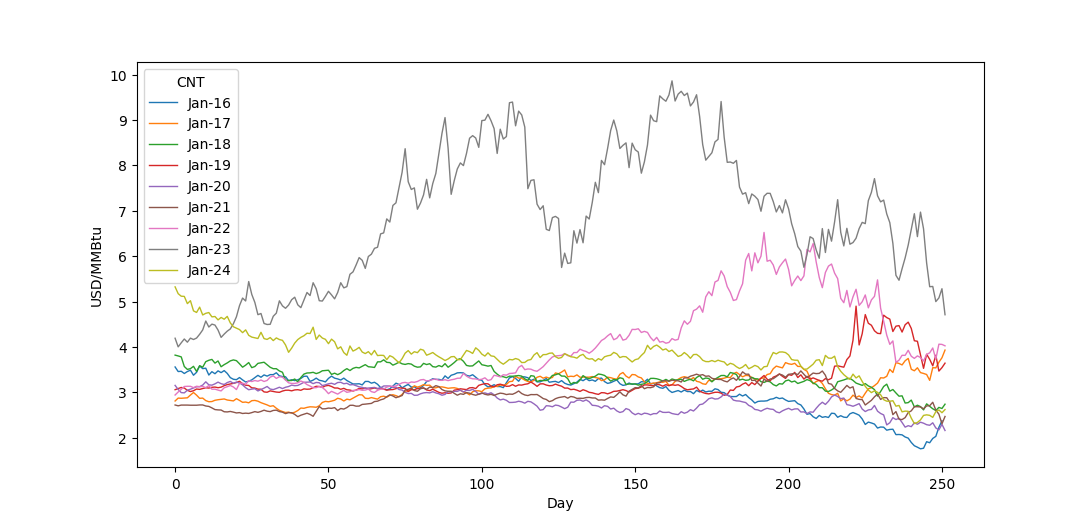
\includegraphics[scale=1,width=1\linewidth,height=0.4\textheight]{Jan_price.png}
\caption{January Futures Contract daily prices within one year before expiry}
\label{JanPrice}
\end{figure}
\begin{figure}[h!] 
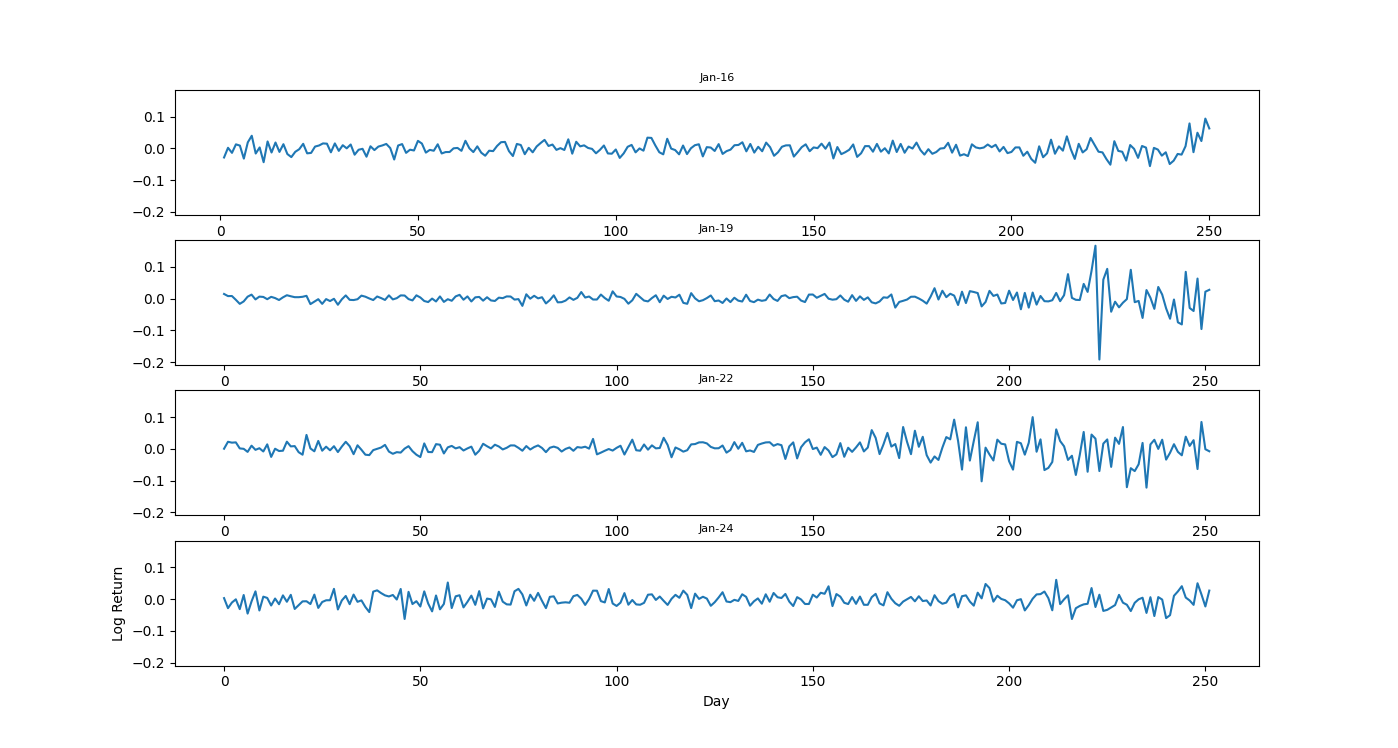
\includegraphics[scale=1,width=1\linewidth,height=0.4\textheight]{Jan_vol.png}
\caption{January Futures Contract daily log return within one year before expiry}
\label{JanVol}
\end{figure}

\colorAutoref{JanHist} depicts the histogram of January contracts' log returns. The heavy-tailed and skewed returns distribution is caused by some large spikes which can be seen in \colorAutoref{JanVol}. As a result, it justifies the application of EGARCH with skewed-t distribution and HESTON models in this study.

\begin{figure}[h!] 
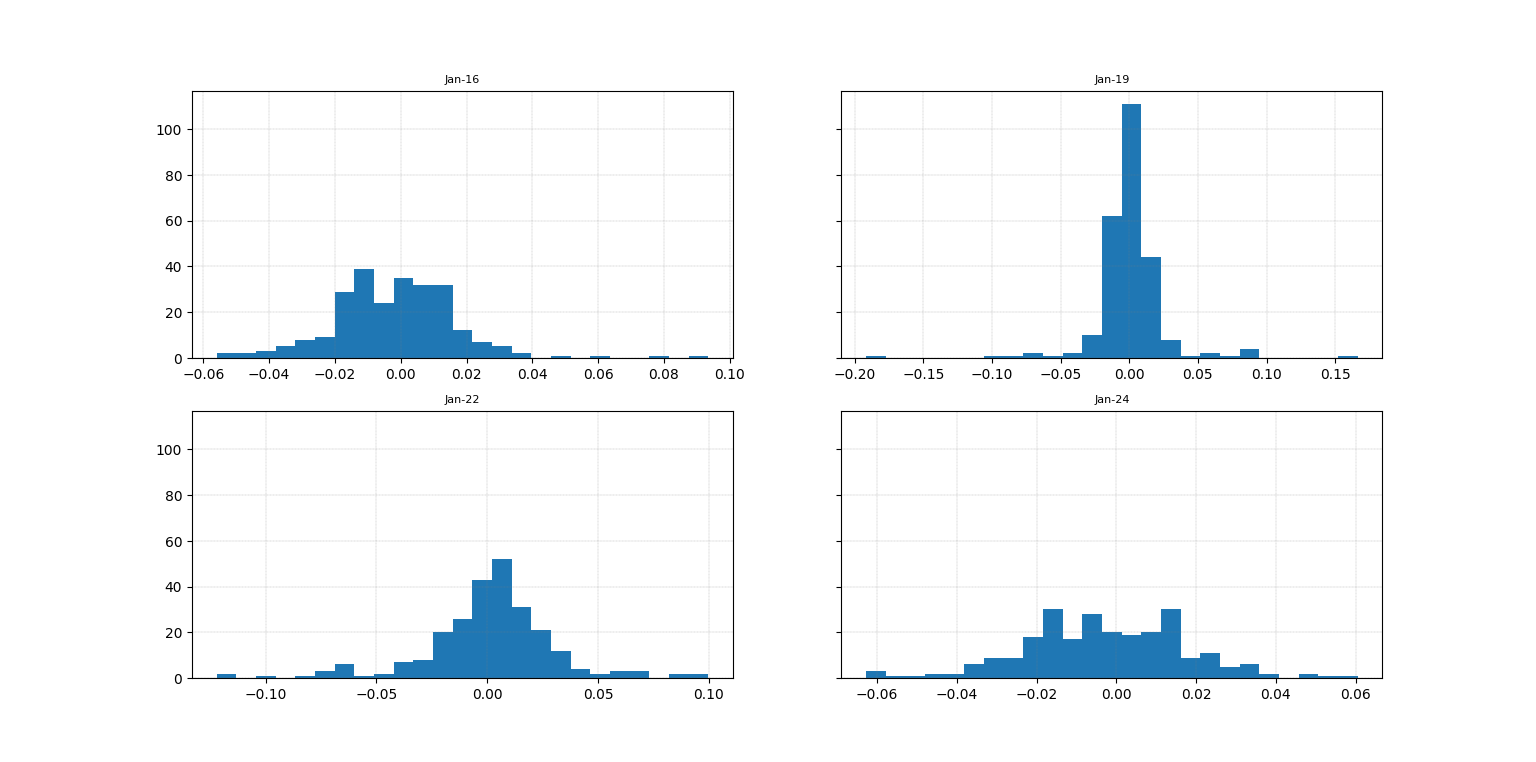
\includegraphics[scale=1,width=1\linewidth,height=0.4\textheight]{Jan_returnshist.png}
\caption{January Futures Contract daily log return histogram}
\label{JanHist}
\end{figure}


\colorAutoref{JulPrice} and \colorAutoref{JulVol} represent the price and log return time series of July contracts. It is noteworthy that Covid 19 seems to not have effect on prices of July 2019 while the political conflict had a significant influence in price of July 2022 and July 2023. On the other hand, volatility cluster is observed for all July 2016, July 2019, July 2022 and July 2024, which is the most important argument for using time-varying volatility models like EGARCH and HESTON.

\begin{figure}[h!] 
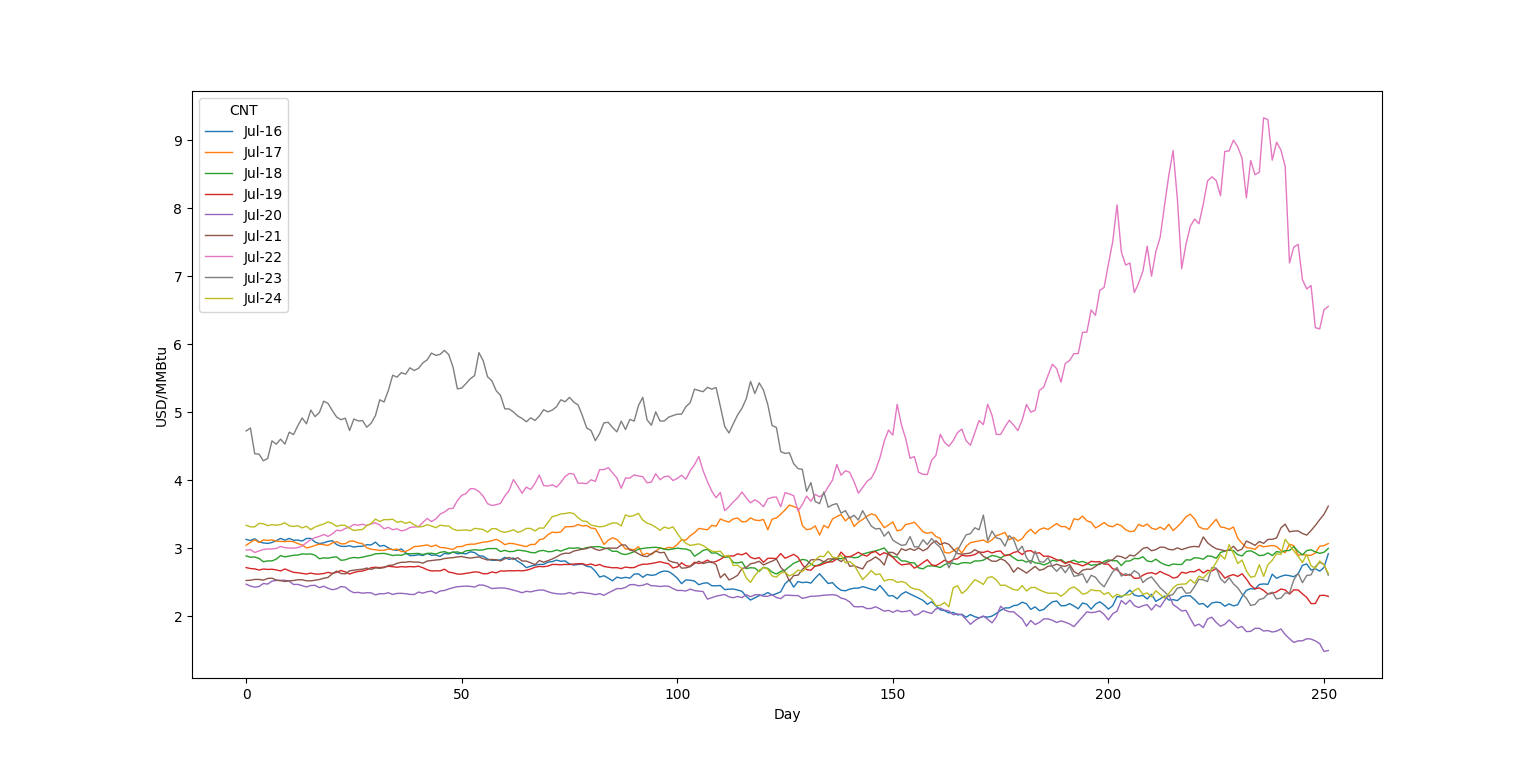
\includegraphics[scale=1,width=1\linewidth,height=0.4\textheight]{Jul_price.png}
\caption{July Futures Contract daily prices within one year before expiry}
\label{JulPrice}
\end{figure}
\begin{figure}[h!] 
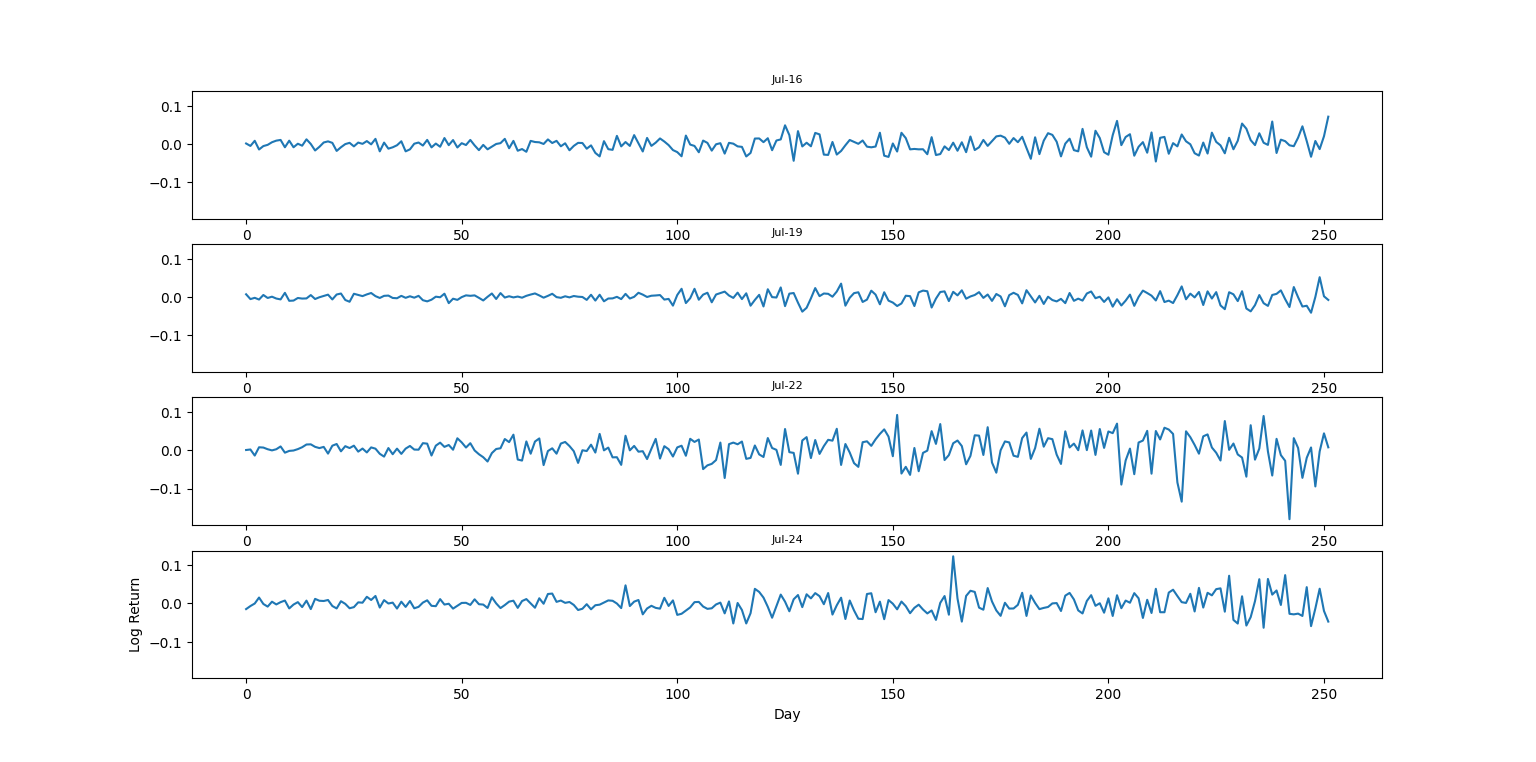
\includegraphics[scale=1,width=1\linewidth,height=0.4\textheight]{Jul_vol.png}
\caption{July Futures Contract daily log return within one year before expiry}
\label{JulVol}
\end{figure}

\colorAutoref{Jan16pacf} shows the sample autocorrelation function (ACF) and partial autocorrelation function (PACF) of January 2016 logarithm return at first moment and second moment. The finding is in line with one of the literature of financial returns' s stylized facts that there is no clear presense of autocorralation of return while there are significant autocorreltion of squared returns. These ACF and PACF features quantitatively indicate the volatility clustering which justifies the used of EGARCH and HESTON models. More graphical illustration for ACF and PACF of other futures contracts can be found in Appendix.

\begin{figure}[h!] 
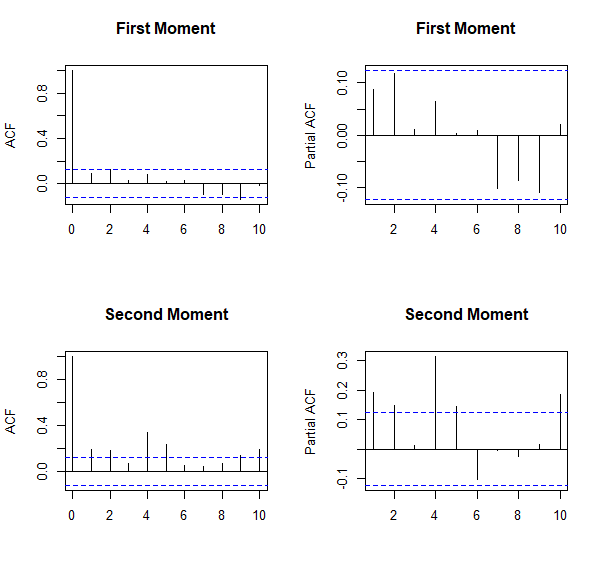
\includegraphics[scale=1,width=1\linewidth,height=0.4\textheight]{Jan16_pacf.png}
\caption{ACF and PACF of January 2016 log return and log return squared}
\label{Jan16pacf}
\end{figure}

In this study, I assume Efficient Market Hypothesis (EMH) holds true that prices fully reflect all available information at any given time. Based on EMH, futures prices are random and there is no need to use past information or exogenous variables to systematically predict prices. Therefore, this study utilizes only prices series, and focus on analyzing its dynamic employing EGARCH and HESTON model.

\section{Methodology}

\subsection{EGARCH}


\subsubsection{Background and motivation}

Traditional econometrics model which assumes homoskedasticity does not represent the well-documented stylized facts of financial time series, such as volatility clustering, leverage effects, and fat-tailed distributions. In 1982, autoregressive conditionally heteroscedastic (ARCH) models was first developed by Engle. The ARCH model is the first formal framework to capture volatility clustering. It describes volatility as a function of past squared residuals (shocks).

While ARCH model is simple and successfully describes the important characteristic of financial returns, it usually requires a large number of lagged squared residuals to sufficiently represent the volatility process, resulting in estimation inefficiency. To address this issue, some alternatives were introduced. An extension of ARCH model, general autoregressive conditionally heteroscedastic (GARCH),  proposed by Bollerslev (1986) is one of the most well-known approach. 

The important feature of (G)ARCH models are the conditional variance, which allows the variance at time t depending on the variances and shocks at time u with $u<t$.

A strong GARCH(p,q) model is given by

 \begin{align*}
 &\epsilon_t = \sigma_t \eta_t,\\[0.6em]
 &\sigma_t^2 = \omega + \sum_{i=1}^p \alpha_i \epsilon_{t-i}^2+ \sum_{j=1}^q \beta_j \sigma_{t-j}^2
 \end{align*}
 
 where the $\alpha_i$ and $\beta_j$ are non-negative constant and $\omega$ is positive constant, and $\eta_t ~ \mathbb{N}(0,1)$.

If all $\beta_j =0$, function of variance becomes


 \begin{align*}
 \sigma_t^2 = \omega + \sum_{i=1}^p \alpha_i \epsilon_{t-i}^2
 \end{align*}
 
 and the process has a form of ARCH(p).
 
As GARCH(p,q) model has ARCH($\infty$); therefore, it helps to capture the process of variance without adding too many lag of shocks and variances. However, there are some technical and practical issues one has to consider when employing GARCH(p,q) to modelling financial volatility cluster.

First, $\alpha_i$ and $\beta_j$ have to be positive to ensure that $\sigma^2 >0$. The restriction makes it hard to have efficient optimizer.

Second, ARCH and GARCH both assume the symmetric effect of negative and positive shock although there is obviously the asymmetric influence of price shocks in practice. 

Exponential general autoregressive conditionally heteroscedastic (EGARCH) is one of the solution to both issue while maintaining the capability to capture volatility clustering.


\subsubsection{EGARCH (1,1) Model}

EGARCH captures volatility clustering as the conditional variance (volatility) is represented by a function of past squared returns, absolute returns, and other variables, in a way that accounts for the persistence of volatility over time. The EGARCH(p,q) model, proposed by Nelson et al. (1991), is defined as follows:

 \begin{align*}
 &r_t = \ln \left(\frac{S_t}{S_{t-1}}\right) = \mu + \epsilon_t ,\\[0.6em]
 &\epsilon_t = \sigma_t z_t,\\[0.6em]
 &\ln\left(\sigma_t^2\right) = \omega + \sum_{i=1}^p \left\{ \alpha_i \left( |z_{t-i}| - \mathbb{E}[|z_{t-i}|] \right) + \gamma_i z_{t-i} \right\} + \sum_{j=1}^q \beta_j \ln\left(\sigma_{t-j}^2\right)
 \end{align*}
 where $S_t$ is natural gas futures price at time t,  $r_t$ represents the logarithmic returns at time t, $\mu$ is the mean of return, $\sigma_t = Var(\epsilon_t|\epsilon_u, u<t)$ is the conditional variance, $z_t$ is an i.i.d standardized residuals (innovations), $\omega$ is constant term, $\alpha_i$ measures the impact of magnitude of past shocks (symmetric effect), $\gamma_i$ represent the sign effect of $z_t$ (asymmetric effect), $\beta_j$ is coefficient of past conditional variances, p and q are the orders of EGARCH model. The term $\sum_{j=1}^q \beta_j \ln\left(\sigma_{t-j}^2\right)$ captures the persistence of volatility. Specifically, high $\beta$ implies that large volatility in previous period tends to result in large volatility in subsequent periods. Since $\ln(\sigma_t^2)$ can be negative, the positivity of the variance is automatically satisfied; therefore, there is no restrictions for parameters.
 
 This thesis considers EGARCH(1,1) in order to have similar model setting with Heston model. The conditional variance of logarithmic returns under EGARCH(1,1) becomes:
 
  \begin{align*}
  \ln\left(\sigma_t^2\right) = \omega + \alpha \left( |z_{t-1}| - \mathbb{E}[|z_{t-1}|] \right) + \gamma z_{t-1} +  \beta \ln\left(\sigma_{t-1}^2\right)
 \end{align*}
By construction, $\gamma z_t$ and $\alpha (|z_t| - \mathbb{E}[|z_t|])$ have mean zero. If the distribution of $z_t$ is symmetric, the two elements are orthogonal. The conditional variance process responds asymmetrically to increase and decrease in price, which can be demonstrated as follows: 
 \begin{equation}
 \begin{cases}
 \ln\left(\sigma_t^2\right) &= \omega + (\alpha + \gamma) z_{t-1} +  \beta \ln\left(\sigma_{t-1}^2\right), 0 < z_t < \infty \\[0.6em]
 \ln\left(\sigma_t^2\right) &= \omega + (-\alpha + \gamma) z_{t-1} +  \beta \ln\left(\sigma_{t-1}^2\right), -\infty < z_t \le 0
 \end{cases}
 \end{equation}

Additionally, $z_t$ is assumed to be skewed-student-t distributed (SST) with mean 0 and variance 1. As a result, $\epsilon_t \sim SST(0, \sigma_t)$. The Student-t distribution is useful in capturing the heavy tails and skewness feature of empirical log-return time series. Developed by Fernandez and Steel in 1998, the density of $SST(\sigma, \nu, \delta)$ is defined as follows:


\begin{align}
f(z|\sigma, \nu, \delta) &= \frac{2}{\delta+ \frac{1}{\delta}} \frac{\Gamma\left(\frac{\nu + 1}{2}\right)}{\Gamma\left(\frac{\nu}{2}\right) \sqrt{\pi \nu}\sigma}
\left[ 1 + \frac{z^2}{\sigma^2 \nu} \left( \frac{1}{\delta^2} \mathbbm{1}_{[0, \infty)} (z) + \delta^2 \mathbbm{1}_{(-\infty, 0)} (z) \right) \right]^{-\frac{\nu + 1}{2}}
\end{align}
\text{with: }
\begin{align}
\nu &>2 \text{ is degree of freedom}, \\
\delta&>0 \text{ represents skewness parameter}\\
\delta^2 &= \frac{P(z \ge 0| \sigma, \nu, \delta)}{P(z < 0| \sigma, \nu, \delta}
\end{align}

If $\delta = 1$, SST is reduced to Student-t distribution, which was developed in Bollerslev (1987). When $\delta  \in (0,1)$, SST is left-skewed, and when $\delta > 1$, SST is right-skewed.

\subsubsection{Estimation}

I consider EGARCH(1,1) model that cover all leverage effect, heavy tail and skew innovation. The proposed model is defined as follow:

\begin{align*}
 &r_t = \ln \left(\frac{S_t}{S_{t-1}}\right) = \mu + \epsilon_t ,\\[0.6em]
 &\epsilon_t = \sigma_t z_t,\\[0.6em]
 &z_t \sim SST(0, 1, \nu, \delta), \\[0.6em]
 &\epsilon_t \sim SST(0, \sigma_t, \nu, \delta), \\[0.6em]
 &\ln\left(\sigma_t^2\right) = \omega + \alpha \left( |z_{t-1}| - \mathbb{E}[|z_{t-1}|] \right) + \gamma z_{t-1} +  \beta \ln\left(\sigma_{t-1}^2\right)
 \end{align*}

The parameter set $ \varphi = (\mu, \alpha, \beta, \gamma, \delta, \nu)$ is estimated using Quasi-Maximum Likelihood (QML) approach (Francq, C. and Zakoian, J. M., 2019). In order to adopt QML, besides the i.i.d skewed-Student-t distribution of innovation $z_t$, some initial values $z_{t-1}, \sigma_{t-1}$  have to be chosen according to the estimated parameters as well as the observed $r_t$, which can be described as follows:

\begin{align}
\sigma_{0} &= \exp \left( \frac{\Tilde{\omega}}{1-\Tilde{\beta}} \right)^{0.5}, \label{eq:3.6}\\[0.6em]
z_{0} &= \frac{r_{0} - \Tilde{\mu}}{\sigma_{0}}
\end{align}

with $\Tilde{\omega} \text{ and } \Tilde{\beta}$ are candidate for estimated parameters. \eqref{eq:3.6} is achieved by assuming $z_t = 0$ and $\sigma_t = \sigma_{t-1}$ in the long-run. Although it is not exact, it would be efficient to have a good initial values which is necessary for QML estimation.

The $\Tilde{\epsilon_t}$, t = 1,..., n, and $\Tilde{\sigma}^2_t$, t = 1,..., n are recursively determined by

\begin{align*}
& \Tilde{\epsilon}_t = r_t - \mu \\[0.6em]
& \Tilde{z}_t = \frac{\Tilde{\epsilon}_t}{\Tilde{\sigma}_t}\\[0.6em]
 &\ln\left(\Tilde{\sigma}_t^2\right) = \Tilde{\omega} + \Tilde{\alpha} \left( |\Tilde{z}_{t-1}| - \mathbb{E}[|\Tilde{z}_{t-1}|] \right) + \Tilde{\gamma} \Tilde{z}_{t-1} +  \Tilde{\beta} \ln\left(\Tilde{\sigma}_{t-1}^2\right)
\end{align*}

The conditional skewed-Student-t quasi-likelihood is as follows

\[L_n(\varphi) = \prod_{t=1}^{n} f(\Tilde{z}_t|1, \Tilde{\nu}, \Tilde{\delta})], \]

with

\[f(\Tilde{z}_t|1, \Tilde{\nu}, \Tilde{\delta}) = \frac{2}{\Tilde{\delta}+ \frac{1}{\Tilde{\delta}}} \frac{\Gamma\left(\frac{\Tilde{\nu} + 1}{2}\right)}{\Gamma\left(\frac{\Tilde{\nu}}{2}\right) \sqrt{\pi \Tilde{\nu}}}
\left[ 1 + \frac{z^2}{\Tilde{\nu}} \left( \frac{1}{\Tilde{\delta}^2} \mathbbm{1}_{[0, \infty)} (\Tilde{z}) + \Tilde{\delta}^2 \mathbbm{1}_{(-\infty, 0)} (\Tilde{z}) \right) \right]^{-\frac{\Tilde{\nu} + 1}{2}}
\]

The QML estimated parameters $\hat{\varphi}$ is achieved by maximize the likelihood $L_n(\varphi)$ or log-likelihood $\ln(L_n(\varphi))$. It is equivalent to minimize the loss function given below

\[\hat{\varphi} = \arg\min_\varphi \left [ - \ln(L_n(\varphi)) \right] \]


\subsection{Heston model}
\subsubsection{Background and motivation}

\textbf{Black-Scholes model}

Black-Scholes model, which assumes Geometric Brownian Motion (GBM) has been become the benchmark of models for financial derivatives pricing. The price of equity or commodity is given by GBM as follows

\begin{align*}
dS_t = \mu S_t dt + \sqrt{V} S_t dW_t^s
\end{align*}

where 

\begin{itemize}
\item $S_t$: asset price at time t
\item $\mu$: expected return
\item $\sqrt{V}$: constant volatility
\item $W_t^s$: Wiener process (Brownian motion)
\end{itemize}

Back-Scholes model is well-known thanks to its closed-form solution for European options pricing. However, it has several issues for practitioners when applying in real world. First, volatility $\sqrt{V}$ is assumed to be constant over time. It can be seen from empirical data that volatility is time-varying and has feature of clustering. Secondly, in real world, volatility tends to revert to long-term mean, but this feature is not covered by GBM either. To address these issues, stochastic volatility Heston models were developed in 1993 where underlying price follows GBM with stochastic volatility be represented by Ornstein-Uhlenbeck process.

\textbf{Ornstein-Uhlenbeck}

The mean reversion Ornstein-Uhlenbeck model is employed in Heston model for describing stochastic volatility process

\begin{align*}
dV_t = \kappa (\theta - V_t) dt + \sqrt{V_t} \sigma_V dW_t^V 
\end{align*}

where 
\begin{itemize}
\item $V_t$: variance at time t
\item $\kappa$: speed of mean reversion
\item $\theta$: long-term volatility
\item $\sigma_V$: volatility of volatility
\item $W_t^v$: Wiener process (Brownian motion)
\end{itemize}

Ornstein-Uhlenbeck process has property of mean reversion that volatility fluctuates but tends to revert to long-term level. Additionally, Brownian motion $W_t^v$ make the process stochastic.


\subsubsection{Model}
The Heston model is an extension of the Black and Scholes model (BSM) that Heston model considers stochastic volatility (Heston 1993). Heston model is given by two stochastic differential equations:

\begin{align}
dS_t &= \mu S_t dt + \sqrt{V_t} S_t dW_t^S \label{eq:3.8} \\[0.6em]
dV_t &= \kappa (\theta - V_t) dt + \sqrt{V_t} \sigma_V dW_t^V \label{eq:3.9} \\[0.6em]
dW_t^S dW_V^2 &= \rho \\[0.6em]
2\kappa \theta &\ge \sigma_V^2 \label{eq:3.10}
\end{align}

with the \eqref{eq:3.8} represents asset price process at time t, and stochastic volatility of asset price is assumed to admit an Ornstein-Uhlenbeck process given in \eqref{eq:3.9} where $\mu$ is growth rate or expected return of asset price, $\theta$ represent the long-term average from which the volatility diverges and to which it then returns $\kappa$ is mean reversion speed coefficient (the larger the k, the longer it takes to return to $\theta$)
$\sigma_V$ is volatility of the volatility, and it is generally responsible for the “scale” of randomness of the volatility process and $dW^S, dW^V$ are two correlated standard Brownian motions with a $\rho \neq 0$ correlation. The Feller condition in \eqref{eq:3.10} ensures the non-negative of variance.

By applying Ito's Lemma, which is discussed in Appendix, Heston model becomes:

\begin{align*}
d \ln(S_t) &= \left( \mu - \frac{1}{2}V_t \right) dt + \sqrt{V_t} dW_t^S \\[0.6em] 
dV_t &= \kappa (\theta - V_t) dt + \sqrt{V_t} \sigma_V dW_t^V \\[0.6em] 
dW_t^1 dW_t^2 &= \rho
\end{align*}

In order to estimate parameter and to forecast the price process, Heston model needs to be discretized. By Euler–Maruyama discretisation scheme (Kloeden and Platen, 1992), Heston model can be described as

\begin{align*}
\ln(S_t) - \ln(S_{t-\Updelta t}) &= \left( \mu - \frac{1}{2}V_{t-\Updelta t} \right) \Updelta t+ \sqrt{V_{t - \Updelta t}} \sqrt{\Updelta t} \epsilon_t^S\\[0.6em]
V_t - V_{t-\Updelta t} &= \kappa (\theta - V_{t- \Updelta t}) \Updelta t + \sqrt{V_{t - \Updelta t}} \sqrt{\Updelta t} \epsilon_t^V \\[0.6em] 
\epsilon_t^S &\sim \mathcal{N}(0, 1)\\[0.6em]
\epsilon_t^V &\sim \mathcal{N}(0, \sigma_V^2)\\[0.6em]
Corr(\epsilon_t^S, \epsilon_t^V) &= \rho
\end{align*}

Consider $\Updelta t = \frac{1}{252}$ where 252 stands for the number of business days in a year, $\ln(S_t) - \ln(S_{t-\Updelta t}) = r_t$ is daily return, and all parameters can be interpreted annually. In order to facilitate the estimation, let $\psi = \rho \sigma_V$ and $\Omega = \sigma_V^2(1-\rho^2)$, Heston model can be illustrated as 

 \begin{align}
r_t &= \left( \mu - \frac{1}{2}V_{t-\Updelta t} \right) \Updelta t+ \sqrt{V_{t - \Updelta t}} \sqrt{\Updelta t} \epsilon_t^S \label{eq:3.12} \\[0.6em] 
V_t &= \kappa \theta \Updelta t + V_{t- \Updelta t} (1 - \kappa \Updelta t)  + \sqrt{V_{t - \Updelta t}} \sqrt{\Updelta t} \epsilon_t^V \label{eq:3.13}
\end{align}

\eqref{eq:3.13} shows that volatility squared $V_t$ is a function of $V_{t-\Updelta_t}$ and other parameters. Therefore, HESTON can capture volatility clustering feature of returns. Furthermore, stochastic volatility setup allows random spike or drop in volatility. As a result, it will increase the probability of extreme movements in price, which then causes heavy-tailed distribution of returns because large price changes occurs more frequently in HESTON model than in standard Black-Scholes model. 

After reorganization, it can be seen that

\begin{align*}
\epsilon_t^S &= \frac{r_t - \mu \Updelta t + \frac{1}{2} V_{t-\Updelta t}}{\sqrt{V_{t-\Updelta t}}\sqrt{\Updelta t}}, \\[0.6em]
\epsilon_t^V &= \frac{V_t - \kappa \theta \Updelta t - (1-\kappa \Updelta t) V_{t-\Updelta t}}{\sqrt{V_{t-\Updelta t}}\sqrt{\Updelta t}},\\[0.6em]
(\epsilon_t^S, \epsilon_t^V) &\sim \mathcal{N}\left( (0,0), \begin{pmatrix}
											1 & \rho \sigma_V\\
											\rho \sigma_V & \sigma_V^2
										    \end{pmatrix} \right) = \mathcal{N} \left((0,0) , \begin{pmatrix}
																				1 & \psi \\
																				\psi  & \psi^2 + \Omega
										    									  \end{pmatrix} \right)
\end{align*}

Over the last decades, parameter estimation for stochastic differential equation has been investigated thoroughly. There are several approaches that have been studied and employed in financial mathematics. According to Gruszka, Jarosław, and Janusz Szwabinski (2023), Bayesian approach performs well in estimating parameters from the model class. In this study, Heston model is estimated by using Markov Chain Monte Carlo (MCMC) method, which bases on Bayesian inference. In general, the prior distribution for each parameter is assumed, then together with data observed, the posterior distribution is formalized. Under the assumption of Markov Chain and the repeated random sampling by Monte Carlo, the estimated parameters are achieved. I briefly discuss the characteristic of Markov Chain and Monte Carlo in the Appendix. The main content solely focus on the prior density assumption and posterior density derivation, which is developed in Joshua Cape et al. (2014).

MCMC distinguishes between parameter set and state space, where parameter set includes $\mu, \kappa, \theta, \sigma_V, \rho$, where state space ${V_0, V_1, ...V_T}$. These two components are estimated jointly using different random sampling methods which are discussed later in this chapter.

\subsubsection{Estimation}
I start with deriving likelihood function of $(r_t, V_t)$. It can be seen from \eqref{eq:3.12} and  \eqref{eq:3.13} that $(r_t, V_t)$ is a linear transformation of $(\epsilon_t^S, \epsilon_t^V)$ respectively. As $(\epsilon_t^S, \epsilon_t^V)$ is jointly normal distributed, $(r_t, V_t)$ follows bivariate normal distribution with joint probability density function given below

\[
P(r, V| \mu, \kappa, \theta, \psi, \Omega) = \Omega^{-n/2} \left( \prod_{t=1}^{n} \frac{1}{V_{t-1}}\right) \exp \left(- \frac{1}{2\Omega} \sum_{t=1}^{n} [(\Omega + \psi^2)(\epsilon_t^S)^2 - 2 \psi \epsilon_t^S \epsilon_t^V + (\epsilon_t^V)^2]\right) \label{eq:3.13}
\]

The joint likelihood of $r_t, V_t$ is then used with the assumptions of prior distribution for parameters to obtain posterior distributions of parameters.

\vspace{1em}

\textbf{A. Posterior distribution of $\mu$}

\vspace{1em}

Assuming that $\mu \sim \mathcal{N}(\mu_0, \sigma_0^2)$, according to Bayes rule, the posterior of $\mu$ is given by

\begin{align*}
P(\mu \mid Y, V, \kappa, \theta, \psi, \Omega) & \propto P(Y, V \mid \mu, \kappa, \theta, \psi, \Omega) \cdot P(\mu) \\[0.6em]
& \propto \exp\left( -\frac{1}{2\Omega} \sum_{t=1}^{n} \left[ (\Omega + \psi^2)(\epsilon_t^S)^2 - 2\psi \epsilon_t^V \epsilon_t^S \right] \right) \cdot \exp\left( -\frac{(\mu - \mu_0)^2}{2\sigma_0^2} \right) \\[0.6em]
& \propto \exp\left( -\frac{1}{2} \sum_{t=1}^{n} \left[ \frac{\Omega + \psi^2}{\Omega} \left( \frac{Y_t - \mu \Delta t + \frac{1}{2} V_{t-1} \Delta t}{\sqrt{V_{t-1} \Delta t}} \right)^2 \right. \right. \\[0.6em]
& \left. \left. - \frac{2\psi}{\Omega} \left( \frac{V_t - \kappa \theta \Delta t - (1 - \kappa \Delta t) V_{t-1}}{\sqrt{V_{t-1} \Delta t}} \right) \left( \frac{-\mu \Delta t}{\sqrt{V_{t-1} \Delta t}} \right) \right] \right) \\[0.6em]
& \cdot \exp\left( -\frac{\mu^2 - 2\mu_0 \mu}{2\sigma_0^2} \right)\\[0.6em]
& \propto\exp\left(-\frac{1}{2} \left[\left(\sum_{t=1}^n \frac{\Omega + \psi^2}{\Omega V_{t-1}}\right) \mu^2 \Delta t \right. \right. \\[0.6em] 
& \left. \left. - 2\sum_{t=1}^T \left(\frac{(\Omega + \psi^2)(Y_t - \frac{1}{2} V_{t-1} \Delta t)}{\Omega V_{t-1} \sqrt{V_{t-1} \Delta t}} - \frac{\psi \left(V_t - \kappa \theta \Delta t - (1 - \kappa \Delta t)V_{t-1} \right)}{\Omega V_{t-1}} \right) \mu \right] \right) \\[0.6em]
& \cdot \exp\left(-\frac{1}{2} \left[\frac{1}{\sigma_0^2} \mu^2 - 2 \frac{\mu_0}{\sigma_0^2} \mu \right] \right).
%%& \propto \exp \left( \frac{-1}{2} \left( \Delta t \sum_{t=1}^n \frac{\Omega + \psi^2}{\Omega V_{t-1}}  + \frac{1}{\sigma_0^2}\right) \right  \right)^{-1} 
\end{align*}

After simplification, the $\mu \sim \mathcal{N}(\mu^*, \sigma^{*2})$ with

\[
\mu^* = \frac{\sum_{t=1}^n ((\Omega + \psi^2) (Y_t + \frac{1}{2} V_{t-1} \Delta t)/\Omega V_{t-1}) - \sum_{t=1}^n (\psi (V_t - \kappa \theta \Updelta t - (1 - \kappa \Updelta t)V_{t-1})/\Omega V_{t-1}) + \mu_0/\sigma_0^2}{\Updelta t \sum_{t=1}^n ((\Omega + \psi^2) / \Omega V_{t-1}) + 1 / \sigma_0^2}
\]

\[
\sigma^{*2} = \frac{1}{\Delta t \sum_{t=1}^n ((\Omega + \psi^2) / \Omega V_{t-1}) + 1 / \sigma_0^2}
\]

\vspace{1em}

\textbf{B. Posterior distribution of $\psi$ and $\Omega$}
\vspace{1em}

Let the prior distribution assumptions be $\Omega\sim \mathcal{IG}(\Tilde{\alpha}, \Tilde{\beta})$ and $\psi_{|\Omega} \sim \mathcal{N}(\psi_0, \Omega/p_0)$. In Bayesian statistics, the inverse gamma distribution is commonly used as a prior for the variance of a normal distribution because it ensures the conjunction property.

First, the joint posterior density of $(\psi,\Omega)$ is as follows

\begin{align*}
P(\psi, \Omega \mid Y, V, \kappa, \theta, \mu) &\propto P(Y, V \mid \psi, \Omega, \kappa, \theta, \mu) \cdot P(\psi \mid \Omega) \cdot P(\Omega) \\[0.6em]
& \propto \Omega^{-T/2} \exp\left( -\frac{1}{2\Omega} \sum_{t=1}^{T} \left[ (\Omega + \psi^2)(\epsilon_t^S)^2 + (\epsilon_t^V)^2 - 2\psi \epsilon_t^S \epsilon_t^V \right] \right) \\[0.6em]
& \cdot \sqrt{\frac{p_0}{\Omega}} \exp\left( -\frac{(\psi - \psi_0)^2}{2\Omega/p_0} \right) \cdot \frac{\tilde{\beta}^{\tilde{\alpha}}}{\Gamma(\tilde{\alpha})} \Omega^{-\tilde{\alpha}-1} \exp\left( -\frac{\tilde{\beta}}{\Omega} \right) \\[0.6em]
& \propto \Omega^{-T/2 - \tilde{\alpha} - 1} \cdot \frac{1}{\Omega^{1/2}} \cdot \exp\left( -\frac{1}{2\Omega} \sum_{t=1}^{T} \left[ (\Omega + \psi^2)(\epsilon_t^S)^2 + (\epsilon_t^V)^2 - 2\psi \epsilon_t^S \epsilon_t^V \right] \right. \\[0.6em]
& \left. - \frac{1}{2} \frac{(\psi - \psi_0)^2}{\Omega/p_0} - \frac{\tilde{\beta}}{\Omega} \right)\\[0.6em]
&\propto \Omega^{-n/2-\Tilde{\alpha}-1} \cdot \exp \left( -\frac{1}{\Omega} \left[\Tilde{\beta} + \frac{1}{2}\sum_{t=1}^n (\epsilon_t^V)^2\right]\right) \cdot \exp \left(\frac{-1}{2\Omega}p_0\psi_0^2\right)\frac{1}{\Omega^{1/2}}\\[0.6em]
&\cdot \exp \left( -\frac{1}{2 \Omega} \left[ \left( p_0 + \sum_{t=1}^n (\epsilon_t^S)^2 \right) \psi^2 -2 \left(p_0 \psi + \sum_{t=1}^n \epsilon_t^S \epsilon_{t=1}^V \right) \psi \right. \right.\\[0.6em]
&\left. \left. + \frac{(p_0 \psi_0 + \sum_{t=1}^n \epsilon_t^S \epsilon_t^V )^2 }{p_0 + \sum_{t=1}^n (\epsilon_t^S )^2 } - \frac{(p_0 \psi_0 + \sum_{t=1}^n \epsilon_t^S \epsilon_t^V )^2 }{p_0 + \sum_{t=1}^n (\epsilon_t^S )^2 }\right]\right)
\end{align*}

Consider the terms only relating to $\Omega$, $\Omega \sim \mathcal{IG}(\alpha_*, \beta_*)$ with

\[\alpha_* = \frac{n}{2} + \Tilde{\alpha}\] 

and 

\[\beta_* = \Tilde{\beta} + \frac{1}{2} \sum_{t=1}^n (\epsilon_t^V)^2 + \frac{1}{2} p_0 \psi_0^2 - \frac{1}{2} \frac{(p_0 \psi_0 + \sum_{t=1}^n \epsilon_t^S \epsilon_t^V)^2}{p_0 + \sum_{t=1}^n (\epsilon_t^S )^2} \] 

Additionally, $\psi_{|\Omega} \sim \mathcal{N} (\psi_*, \sigma_\psi^{*2})$ where

\[\psi_* =\frac{(p_0 \psi_0 + \sum_{t=1}^n \epsilon_t^S \epsilon_t^V)^2}{p_0 + \sum_{t=1}^n (\epsilon_t^S )^2} \]

and 

\[\sigma\psi^{*2} = \frac{\Omega}{p_0 + \sum_{t=1}^n (\epsilon_t^S)^2 }\]

\vspace{1em}

\textbf{C. Posterior distribution of $\theta$}

\vspace{1em}

Assume that the prior of $\theta \sim \mathcal{N}(\theta_0, \sigma_\theta^2)$, then the posterior of $\theta$ is given by

\begin{align*}
P(\theta \mid Y, V, \mu, \kappa, \psi, \Omega) & \propto P(Y, V \mid \mu, \kappa, \theta, \psi, \Omega) \cdot P(\theta) \\[0.6em]
& \propto \exp\left( -\frac{1}{2\Omega} \sum_{t=1}^{T} \left[ (\epsilon_t^V)^2 - 2\psi \epsilon_t^V \epsilon_t^S \right] \right) \cdot \exp\left( -\frac{(\theta - \theta_0)^2}{2\sigma_\theta^2} \right)\\
& \propto \exp\left( -\frac{1}{2} \sum_{t=1}^{T} \left[ \frac{1}{\Omega} \left( \frac{V_t - \kappa \theta \Delta t - (1 - \kappa \Delta t)V_{t-1}}{\sqrt{V_{t-1} \Delta t}} \right)^2 \right. \right. \\
& \left. \left. - \frac{2\psi}{\Omega} \left( \frac{Y_t - \mu \Delta t + \frac{1}{2} V_{t-1} \Delta t}{\sqrt{V_{t-1} \Delta t}} \right) \left( \frac{-\kappa \theta \Delta t}{\sqrt{V_{t-1} \Delta t}} \right) \right] \right) \\
& \cdot \exp\left( -\frac{\theta^2 - 2\theta_0 \theta}{2\sigma_\theta^2} \right)\\
& \propto\exp\left(-\frac{1}{2} \left[\left(\sum_{t=1}^n \frac{\kappa^2}{\Omega V_{t-1}}\right) \theta^2 \Delta t \right. \right. \\[0.6em] 
& \left. \left. - 2\sum_{t=1}^T \left(\frac{\kappa (V_t - (1-\kappa \Delta t) V_{t-1})}{\Omega V_{t-1}} - \frac{\psi (r_t -\mu \Updelta t + \frac{1}{2} V_{t-1} \Updelta t) \kappa}{\Omega V_{t-1}} \right) \theta \right] \right) \\[0.6em]
& \cdot \exp\left(-\frac{1}{2} \left[\frac{1}{\sigma_\theta^2} \theta^2 - 2 \frac{\theta_0}{\sigma_\theta^2} \theta \right] \right).
\end{align*}

It requires some more reorganization to see that $\theta \sim \mathcal{N}(\theta^*, \sigma_\theta^2)$ with

\[
\theta^* = \frac{\sum_{t=1}^n (\kappa (V_t - (1-\kappa \Delta t) V_{t-1}))/\Omega V_{t-1}) - \sum_{t=1}^n (\psi (V_t - \kappa \theta \Updelta t - (1 - \kappa \Updelta t)V_{t-1})/\Omega V_{t-1}) + \theta_0/\sigma_\theta^2}{\Updelta t \sum_{t=1}^n (\kappa^2 / \Omega V_{t-1}) + 1 / \sigma_\theta^2}
\]
and
\[
\sigma^{*2} = \frac{1}{\Delta t \sum_{t=1}^n (\kappa^2 / \Omega V_{t-1}) + 1 / \sigma_\theta^2}
\]

\textbf{Posterior distribution of $\kappa$}

Let $\kappa \sim \mathcal{N}(\kappa_0, \sigma_\kappa^2)$, similarly the posterior density is as follows

\begin{align*}
P(\kappa \mid Y, V, \mu, \theta, \psi, \Omega) & \propto P(Y, V \mid \mu, \kappa, \theta, \psi, \Omega) \cdot P(\kappa) \\[0.6em]
&\propto \exp\left(-\frac{1}{2\Omega} \Sigma_{i=1}^T [(\epsilon_i^V)^2 - 2\psi \epsilon_i^V \epsilon_i^S]\right) \cdot \exp\left(-\frac{(\kappa - \kappa_0)^2}{2\sigma_k^2}\right) \\[0.6em]
&\propto \exp\left(-\frac{1}{2} \Sigma_{i=1}^T \left[ \frac{1}{\Omega} \left( \frac{V_t - \kappa \theta \Delta t - (1 - \kappa \Delta t) V_{t-1}}{\sqrt{V_{t-1} \Delta t}} \right)^2 \right. \right. \\[0.6em]
& \left. \left.  - \frac{2\psi}{\Omega} \left( \frac{V_t - \mu \Delta t + \frac{1}{2} V_{t-1} \Delta t}{\sqrt{V_{t-1} \Delta t}} \right) \left( -\frac{\kappa (\theta - V_{t-1}) \Delta t}{\sqrt{V_{t-1} \Delta t}} \right) \right] \right) \\[0.6em]
& \cdot \exp\left(-\frac{(\kappa^2 - 2\kappa_0 \kappa)}{2\sigma_k^2}\right)\\[0.6em]
& \propto\exp\left(-\frac{1}{2} \left[\left(\sum_{t=1}^n \frac{(V_{t-1} - \theta)^2}{\Omega V_{t-1}} \right) \kappa^2 \Updelta t \right. \right. \\[0.6em] 
& \left. \left. - 2\sum_{t=1}^T \left( \frac{(\theta - V_{t-1}) (V_t - V_{t-1})}{\Omega V_{t-1}} - \frac{\psi (r_t - \mu \Updelta t + \frac{1}{2} V_{t-1} \Updelta t )(\theta - V_{t-1})}{\Omega V_{t-1}} \right) \kappa \right] \right) \\[0.6em]
& \cdot \exp\left(-\frac{1}{2} \left[\frac{1}{\sigma_\kappa^2} \kappa^2 - 2 \frac{\kappa_0}{\sigma_\kappa^2} \kappa \right] \right).
\end{align*}

After some transformations, posterior distribution of $\kappa \sim \mathcal{N}(\kappa_*, \sigma_\kappa^*)$ with

\[
\kappa^* = \frac{\sum_{t=1}^n ((\theta - V_{t-1}) (V_t - V_{t-1})/\Omega V_{t-1}) - \sum_{t=1}^n (\psi (r_t - \mu \Updelta t + \frac{1}{2} V_{t-1} \Updelta t )(\theta - V_{t-1})/\Omega V_{t-1}) + \kappa_0/\sigma_\kappa^2}{\Updelta t \sum_{t=1}^n ((V_{t-1}-\theta)^2/\Omega V_{t-1}) + 1 / \sigma_\kappa^2}
\]
and
\[
\sigma_\kappa^{*2} = \frac{1}{\Updelta t \sum_{t=1}^n ((V_{t-1}-\theta)^2/\Omega V_{t-1}) + 1 / \sigma_\kappa^2}
\]

\vspace{1em}

\textbf{Posterior distribution of $V_t$}
\vspace{1em}

\begin{align*}
P(V_t \mid Y, V_{t+1}, V_{t-1}, \kappa, \mu, \theta, \psi, \Omega) &= P(Y, V_{t+1}, V_{t}, \mid V_{t-1}, \mu, \kappa, \theta, \psi, \Omega) \frac{P(V_{t-1} \mid \kappa, \theta, \psi, \Omega, \mu)}{P(r, V_{t+1}, V_{t-1} \mid \kappa, \theta, \psi, \Omega, \mu)}\\[0.6em]
& \propto P(Y, V_{t+1}, V_{t} \mid V_{t-1}, \kappa, \theta, \psi, \Omega, \mu)\\[0.6em]
&\propto \frac{1}{V_t\Delta t}\exp\left(-\frac{1}{2\Omega}\left[(\Omega+\psi^2)(\epsilon_{t+1}^S)^2 - 2\psi\epsilon_{t+1}^S\epsilon_{t+1}^V + (\epsilon_{t+1}^V)^2\right]\right. \\
&\quad \left. -\frac{1}{2\Omega}\left[(\Omega+\psi^2)(\epsilon_i^S)^2 - 2\psi\epsilon_i^S\epsilon_i^V + (\epsilon_i^V)^2\right]\right)\\
&=\frac{1}{V_t \Updelta t}\exp\left(-\frac{1}{2 \Omega} \frac{(\Omega + \psi^2)(\frac{1}{2}V_t \Updelta t + Y_{t+1} - \mu \Updelta t)^2}{V_t \Updelta t} \right. \\[0.6em] 
&= \frac{1}{V_t \Delta t} \exp \left( - \frac{1}{2 \Omega} \frac{(\Omega + \psi^2)\left(\frac{1}{2} V_t \Delta t + Y_{t+1} - \mu \Delta t\right)^2}{V_t \Delta t} \right) \\
&\quad - \frac{1}{2 \Omega} \frac{- 2 \psi \left(\frac{1}{2} V_t \Delta t + Y_{t+1} - \mu \Delta t\right) \left(- (1 - \kappa \Delta t) V_t - \kappa \theta \Delta t + V_{t+1}\right)}{V_t \Delta t} \\
&\quad - \frac{1}{2 \Omega} \frac{\left(- (1 - \kappa \Delta t) V_t - \kappa \theta \Delta t + V_{t+1}\right)^2}{V_t \Delta t} \\
&\quad - \frac{1}{2 \Omega} \frac{- 2 \psi \left(Y_t - \mu \Delta t + \frac{1}{2} V_{t-1} \Delta t\right) \left(V_t - \kappa \theta \Delta t - (1 - \kappa \Delta t) V_{t-1}\right)}{V_{t-1} \Delta t} \\
&\quad - \frac{1}{2 \Omega} \frac{\left(V_t - \kappa \theta \Delta t - (1 - \kappa \Delta t) V_{t-1}\right)^2}{V_{t-1} \Delta t}
& \left. -\frac{1}{2 \Omega} \frac{-2\psi (\frac{1}{2}V_t \Updelta t + r_{t+1} -mu \Updelta t)(-(1-\kappa \Updelta t)V_t -\kappa \theta \Updelta t + V_{t+1})}{V_t \Updelta t} \right. \\[0.6em]
& \left. -\frac{1}{2 \Omega} \frac{(-(1-\kappa \Updelta t) V_t - \kappa \theta \Updelta t + V_{t+1})^2}{V_t \Updelta t} \right) \\[0.6em]
& \cdot \exp \left( - \frac{1}{2 \Omega} \frac{-2 \psi (Y_t - \mu \Updelta t + \frac{1}{2}V_{t-1} \Updelta t)(V_t - \kappa \theta \Updelta t - (1-\kappa \theta)V_{t-1})}{V_{t-1} \Updelta t} \right. \\[0.6em]
& \left. -\frac{1}{2 \Omega} \frac{(V_t - \kappa \theta \Updelta t - (1-\kappa\Updelta t)V_{t-1})^2}{V_{t-1}\Updelta t}\right).
\end{align*}

\subsubsection{MCMC}

In general, MCMC generates random samples from a given target distribution. In this study, a sequence of sampling of target parameters $\mu, \kappa, \theta, \psi, \Omega$ and space $V_1, V_2, ..., V_n$ are generated based on posterior distributions which are derived from prior distribution assumption and observed data. By construction, the sequence has Markov's properies includin convergence. 
 
According to Michael Johannes and Nicholas Polson (2003), convergence of the sequence relied on the ergodic theory for Markov Chain. A g-step transition probability plays a key role to define a Markov Chain:

\[P^{(g)} (x, A) = P[\theta^{(g)} \in A \mid \theta^0 = x]\]

There are two important conditions for Markov Chain to converge, i.e. irreducible and aperiodic. A Markov chain is irreducible if it has positive probability of eventually entering any set which has $\pi-$positive probability regardless of its initial state. A chain is aperiodic if there are no portions of the state space that the chain visits at regularly spaced time intervals. When two conditions are met, the equilibrium distribution of the chain can be achieved:

\[\lim_{g\rightarrow \infty} P[\theta^{(g)} \in A  \mid \theta^{(0)} ] = \pi(A)\]

It can be seen from the equation that the chain will converge regardless the innital state. This study assume the convergence of estimated parameters after g-steps sampling. While the convergence condition is hard to verified, it is investigated through graphical illustration in this study by tracking the value of sampling each step.

After defining prior distribution and deriving posterior density of parameters set $\mu, \kappa, \theta, \rho$ and state space $V_t$, MCMC is employed to obtained draws from posterior distribution. MCMC approaches utilized for parameters and state space are different. In order to estimate parameters $\mu, \kappa, \theta, \rho$, Gibbs sampler is useful because the posterior distributions are normal distribution and inversed gamma distribution which are well-known and straightforward to sample conditioned on other parameters. Gibbs sampler is the simplest MCMC algorithm that was introduced in Geman and Geman (1984). 

The procedure of Gibbs sampler for parameter set starts with initializing a set of values $\Theta = { \mu^{(0)}, \kappa^{(0)}, \theta^{(0)}, \psi^{(0)}, \Omega^{(0)}, V_0^{(0)}, V_1^{(0)}, ..., V_n^{(0)} }$. First, the distribution of $\mu$ is identified by density mentioned above and these initial values, then a sampling $\mu^{(1)}$ can be obtained from this posterior distribution of $\mu$. Parameter set now is updated to $\Theta = { \mu^{(1)},\psi^{(0)}, \Omega^{(0)}, \kappa^{(0)}, \theta^{(0)}, V_0^{(0)}, V_1^{(0)}, ..., V_n^{(0)} }$. The same process will be applied to obtain draws of $\psi^{(1)}$ and $\Omega^{(1)}$, and  $\Theta = { \mu^{(1)},\psi^{(1)}, \Omega^{(1)}, \kappa^{(0)}, \theta^{(0)}, V_0^{(0)}, V_1^{(0)}, ..., V_n^{(0)} }$. $\kappa^{(1)}$ and $\theta^{(1)}$ can be acquired by following steps mentioned above. 

Unlike parameters sampling that can be obtained easily with Gibbs sampler, the distribution of state space $V = V_0, V_1, ..., V_n$ is not straightforward to simulate. In this case, a random walk Metropolis-Hastings approach is approriate Joshua Cape et al. (2014). Similarly, the algorithm starts with initializing values for 0th step:
\[V_0^{(0)}, V_1^{(0)}, ..., V_n^{(0)}\].

For $g \in {1, 2, ... G}$, after drawing parameters using Gibbs sampler, the algorithm is run to obtain \[V_0^{(g)}, V_1^{(g)}, ..., V_n^{(g)}\]. Specifically, $V_t^{(g)}$ for $t \in {1, 2, ..., n}$ is generating as follows:

\[V_t^{*(g)} = V_t^{(g-1)} + \epsilon_t^V, \text{ with } \epsilon_t^V \sim \mathcal{N}(0, \sigma_V^2)\]
where $t \in {1, 2, ..., n}$ and $V_t^{*(g)}$ is new proposal for $V_t^{(g)}$. $\sigma_V^2$ is volatility of volatility. 

New proposal $V_t^{(g)}$ is rejected or accepted based on the comparison of likelihood of $V_t^{(g-1)}$ and new one. The computation of acceptance rate for new proposal is given by:

\[\mathcal{A}(V_t^{*(g)}, V_t^{(g-1)}) = min \left( \frac{\pi(V_t^{*(g)})}{\pi(V_t^{(g-1)})}, 1 \right)\]. 

where $\pi(V_t^{*(g)})$ and $\pi(V_t^{(g-1)})$ are likelihood calculated as follows:

\begin{align*}
\pi(V_t^{*(g)}) &= \frac{1}{V_t^{*(g)} \Updelta t} \exp \left( -\frac{1}{2 \Omega} \frac{(\Omega + \psi^2)(\frac{1}{2} V_t^{*(g)} \Updelta t + Y_{t+1} - \mu \Updelta t)^2)}{V_t^{*(g)} \Updelta t} \right.\\[0.6em]
& \left. -\frac{1}{2\Omega}\frac{-2\psi (\frac{1}{2}V_t^{*(g)} \Updelta t + Y_{t+1} - \mu \Updelta t)(-(1-\kappa\Updelta t) V_t^{*(g)} -\kappa \theta \Updelta t + V_{t+1}^{(g-1)})}{V_t^{*(g)} \Updelta t} \right.\\[0.6em]
& \left. -\frac{1}{2\Omega}\frac{(-(1-\kappa \Updelta t) V_t^{*(g)} -\kappa \theta \Updelta t + V_{t+1}^{*(g-1)})^2}{V_t^{*(g)} \Updelta t} \right)\\[0.6em]
& \cdot \exp \left( - \frac{1}{2 \Omega} \frac{-2 \psi (Y_t - \mu \Updelta t + \frac{1}{2}V_{t-1}^{(g)} \Updelta t)(V_t^{*(g)} - \kappa \theta \Updelta t - (1-\kappa \theta)V_{t-1})}{V_{t-1}^{(g)} \Updelta t} \right. \\[0.6em]
& \left. -\frac{1}{2 \Omega} \frac{(V_t^{*(g)} - \kappa \theta \Updelta t - (1-\kappa\Updelta t)V_{t-1}^{(g)})^2}{V_{t-1}^{(g)}\Updelta t}\right).
\end{align*}

and 

\begin{align*}
\pi(V_t^{(g-1)}) &= \frac{1}{V_t^{(g-1)} \Updelta t} \exp \left( -\frac{1}{2 \Omega} \frac{(\Omega + \psi^2)(\frac{1}{2} V_t^{(g-1)} \Updelta t + Y_{t+1} - \mu \Updelta t)^2)}{V_t^{(g-1)} \Updelta t} \right.\\[0.6em]
& \left. -\frac{1}{2\Omega}\frac{-2\psi (\frac{1}{2}V_t^{(g-1)} \Updelta t + Y_{t+1} - \mu \Updelta t)(-(1-\kappa\Updelta t) V_t^{(g-1)} -\kappa \theta \Updelta t + V_{t+1}^{(g-1)})}{V_t^{(g-1)} \Updelta t} \right.\\[0.6em]
& \left. -\frac{1}{2\Omega}\frac{(-(1-\kappa \Updelta t) V_t^{(g-1)} -\kappa \theta \Updelta t + V_{t+1}^{(g-1)})^2}{V_t^{(g-1)} \Updelta t} \right)\\[0.6em]
& \cdot \exp \left( - \frac{1}{2 \Omega} \frac{-2 \psi (Y_t - \mu \Updelta t + \frac{1}{2}V_{t-1}^{(g)} \Updelta t)(V_t^{(g-1)} - \kappa \theta \Updelta t - (1-\kappa \theta)V_{t-1})}{V_{t-1}^{(g)} \Updelta t} \right. \\[0.6em]
& \left. -\frac{1}{2 \Omega} \frac{(V_t^{(g-1)} - \kappa \theta \Updelta t - (1-\kappa\Updelta t)V_{t-1}^{(g)})^2}{V_{t-1}^{(g)}\Updelta t}\right).
\end{align*}

$\mathcal{A}(V_t^{*(g)}, V_t^{(g-1)})$ then is compared with random sampling U from $\mathcal{U}[0, 1]$. Intuitively, the probability of acceptance equals $\mathcal{A}(V_t^{*(g)}, V_t^{(g-1)})$. The acceptane/rejection decision rule is described as

\begin{align*}
&\text{If } U< \mathcal{A}(V_t^{*(g)}, V_t^{(g-1)}), \text{ then } V_t^{(g)} = V_t^{*(g)},\\
&\text{Otherwise, }  V_t^{(g)} = V_t^{(g-1)}
\end{align*} 

Metropolis-Hastings sampling is iterated for $t \in {1, 2, ..., n}$ in order to determine state space $V_1^{(g)}, V_2^{(g)}, ...V_n^{()}$. For $V_0^{(g)}$, the $\pi(V_0^{*(g)}$ and $\pi(V_0^{(g-1)}$ is computed considering only the first exponential part. 

\begin{align*}
\pi(V_0^{*(g)}) &= \frac{1}{V_0^{*(g)} \Updelta t} \exp \left( -\frac{1}{2 \Omega} \frac{(\Omega + \psi^2)(\frac{1}{2} V_0^{*(g)} \Updelta t + Y_{1} - \mu \Updelta t)^2)}{V_0{*(g)} \Updelta t} \right.\\[0.6em]
& \left. -\frac{1}{2\Omega}\frac{-2\psi (\frac{1}{2}V_0^{*(g)} \Updelta t + Y_{1} - \mu \Updelta t)(-(1-\kappa\Updelta t) V_0^{*(g)} -\kappa \theta \Updelta t + V_{1}^{(g-1)})}{V_0^{*(g)} \Updelta t} \right.\\[0.6em]
& \left. -\frac{1}{2\Omega}\frac{(-(1-\kappa \Updelta t) V_0^{*(g)} -\kappa \theta \Updelta t + V_{1}^{*(g-1)})^2}{V_0^{*(g)} \Updelta t} \right)
\end{align*}

and 

\begin{align*}
\pi(V_0^{(g-1)}) &= \frac{1}{V_0^{(g-1)} \Updelta t} \exp \left( -\frac{1}{2 \Omega} \frac{(\Omega + \psi^2)(\frac{1}{2} V_0^{(g-1)} \Updelta t + Y_{1} - \mu \Updelta t)^2)}{V_0^{(g-1)} \Updelta t} \right.\\[0.6em]
& \left. -\frac{1}{2\Omega}\frac{-2\psi (\frac{1}{2}V_0^{(g-1)} \Updelta t + Y_{1} - \mu \Updelta t)(-(1-\kappa\Updelta t) V_0^{(g-1)} -\kappa \theta \Updelta t + V_{1}^{(g-1)})}{V_0^{(g-1)} \Updelta t} \right.\\[0.6em]
& \left. -\frac{1}{2\Omega}\frac{(-(1-\kappa \Updelta t) V_0^{(g-1)} -\kappa \theta \Updelta t + V_{1}^{(g-1)})^2}{V_0^{(g-1)} \Updelta t} \right)
\end{align*}


\subsection{Evaluation Measurement}

\subsubsection{Continuous ranked probabilistic score}
While mean square error (MSE) or mean absolute error (MAE) is popular when it comes to evaluation of forecast accuracy, probabilistic forecast, which provides forecasts for future and suitable measures of the uncertainty associated with them, requires different criteria to assess the performance of forecasters. Scoring rules play an essential role in both forecast quality measure (Gneiting, T., and  Raftery, A. E., 2007). In some fields, researchers refer the evaluation task served by scoring rules as forecast verification. Specifically, scoring rules provide a single numerical score based on the forecast curve and the actual value. In this paper, continuous ranked probabilistic score (CRPS), which is derived based on predictive cumulative distribution functions, is an appropriate measure for prediction performance for several reasons. First, the forecast density is illustrated in terms of samples by monte carlo simulation. Second, CRPS takes the distance of forecasts and actual value into account by giving credit for assigning high probabilities to values close to the real value. 

Introduced in Gneiting and  Raftery (2007), Let X be a random variable, F be the cumulative distribution function (CDF) of X, such as $F(y) = P [X \leq y]$, x be the observation and F be the CDF associated with an empirical probabilistic prediction, CPRS is defined as follows

\[CRPS(F,x) = - \int_{-\infty}^{\infty}  (F(y) - \mathbb{I}_{(y \geq x)}) ^2 \,dy\]

$\mathbb{I}$ is the indicator function that attains:

\begin{equation*}
\begin{cases}
\mathbb{I}_{(y \geq x)} &= 1, if y \geq x\\
\mathbb{I}_{(y \geq x)} &= 0, if y < x
\end{cases}
\end{equation*}

CRPS can be equivalently written as 

\[CRPS(F, x) =  \frac{1}{2} E_F [|X-X'|] - E_F [|X-x|],\]
 where $X$ and $X'$ are independent samples of random variable with distribution function $F$, $x$ is the observed value.
 
 Moreover, CRPS can usually computed in a closed form. For example, the CPRS of predictive density which is Gaussian distributed $\mathcal{N}(\mu, \sigma^2)$
 
 
 \[CRPS(\mathcal{N}(\mu, \sigma^2), x) = \sigma\left[\frac{1}{\pi} - 2 \varphi \left( \frac{x-\mu}{\sigma} \right) - \frac{x-\mu}{\sigma} \left( 2 \Phi \left( \frac{x-\mu}{\sigma} \right) -1 \right)\right]\]
 
 with $\varphi$ and $\Phi$ is the probability density function and cumulative distribution function of a standard Gaussian distribution respectively. 
 
In addition, CRPS is usually utilized with negative orientation as follows

\[CRPS^*(F, x) = - CRPS(F, x) = E_F |X-x| - \frac{1}{2} E_F |X-X'|\]

The lower the $CRPS^*$ is, the better the forecast is. Negative orientation version is more popular in practice because it not only provide the computation in the same unit as observation that make the $CRPS^*$ easier to interpret. $CRPS^*$ is reduced to MAE if F is a deterministic forecast (point forecast with probability 1):

\[CRPS^*(\hat{X}, x) = E[ | \hat{X} - x | ]\] 

In case of evaluation samples instead of density, $CRPS^*$ can be simply estimated as follows
\[ CRPS^*(F, x) = \frac{1}{m} \sum_{i = 1}^{m} | X_i - x | - \frac{1}{2m^2} \sum_{i = 1}^{m} \sum_{j = 1}^{m} | X_i - X_j |,\]
 where x is observed value, F denotes forecast distribution given m discrete sample $X_1, ..., X_m$.
 
\begin{figure}[h!] 
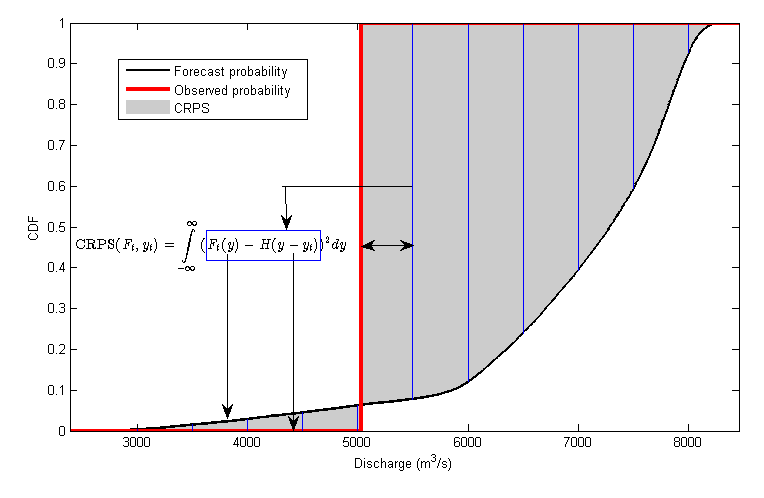
\includegraphics[scale=1,width=1\linewidth,height=0.4\textheight]{CRPS_graphical.png}
\caption{CPRS graphical illustration - Source: Durga Lal Shrestha (MATLAB)}
\label{CRPS_graph}
\end{figure}

The intuition of CRPS is clearly illustrated in \colorAutoref{CRPS_graph}. In real life, only one value x is observed, then the observed probability density function is 

\begin{equation*}
P(y) = 
\begin{cases}
 1, & y = y_t \\
 0 & otherwise
\end{cases}
\end{equation*}

Consequently, observed CDF becomes

\begin{equation*}
F(y) = 
\begin{cases}
 0, & y < y_t \\
 1, & y \geq y_t
\end{cases}
\end{equation*}
 
Put simply, it is shown in \colorAutoref{CRPS_graph} that CRPS represents the gray area between the forecast CDF and observed CDF.The smaller the area, the more accurate the probabilistic forecast. 

In this thesis, forecast accuracy of Heston and EGARCH models are investigated using CRPS. A comparative analysis is conducted not only descriptively but also via hypothesis testing. In order to statistically compare the performance of 2 models, Wilcoxon signed-rank test, which is an alternative for t-test when the normal distribution assumption does not hold, is employed to analyze if one of the two models perform significantly better than the other one. The normal distributed assumption is replaced by a weaker assumption that the difference between the performances of 2 models is symmetric around its mean. Wilcoxon signed-rank test then investigates if the central value is significantly different from zero.

Wilcoxon signed-rank test evaluates the median difference between CRPS of Heston and EGARCH models with the hypothesis as follows

\begin{itemize}
\item Null hypothesis (H0): The median difference between CRPSs of Heston and EGARCH is zero. None of the two models performs better than the other.

\item Alternative hypothesis (H1): The median difference is not zero. There is significant difference in the models' performance.
\end{itemize}



\subsection{Forecasting design}

The analysis including parameterization and forecasting performance of the models was conducted for each futures contract. Specifically, the analysis was performed 2 times for each contract: once 3 months before the expiry and 1 month before the expiry $T$. The estimation window is fixed to 3 months data $S_{T-6*30}$ to $S_{T-3*30}$ for 3 month-ahead forecast and $S_{T-4*30}$ to $S_{T-1*30}$ for 1 month-ahead forecast. Then CPRS was computed using the model forecasts and price at expiry.

EGARCH is estimated by minimizing their negative log-likelihood while Markov Chain Monte Carlo was used to estimate Heston. I implemented them in Python and made used of some built-in packages like pandas, numpy, scipy, SST distribution (Berrisch, 2021). The procedure of parameter estimation and probabilistic forecast is as follows:

\subsubsection{EGARCH}

For each futures contract:

\begin{itemize}
\item EGARCH(1,1) is fitted for financial series of 3 months using MLE approach by minimizing negative log likelihood in equation (3.2) to obtain $ \hat{\varphi} = (\hat{\mu}, \hat{\alpha}, \hat{\beta}, \hat{\gamma}, \hat{\delta}, \hat{\nu})$ only once.
\item Initial volatility is computed as $\sigma_0 = (e^{\frac{\hat{\omega}}{1-\hat{\beta}}})^{0.5}$
\end{itemize}

For i from 0 to 25*3 (for 3 month-ahead forecast) or i from 0 to 25 (for 1 month-ahead forecast)
\begin{itemize}
\item Sampling 1000 i.i.d random variable from skewed Student-t distribution SST(mean = 0, variance = 0, skew = $\hat{\delta}$, degree of freedom = $\hat{\nu}$).
\item Computing
\end{itemize}


\section{Empirical Analysis}

\subsection{Model diagnostics}

\subsubsection{Estimated parameters}

Followed the estimation method outlined in methodology chapter, the parameters are estimated for both models for 3-month and 1-month-ahead forecast. This thesis focuses on comparing the forecast performance of Heston and EGARCH model; however, it is also essential to validate the parameters estimation and in-sample fitted values.

 \colorAutoref{3Mhestonparams} and  \colorAutoref{1Mhestonparams} shows the time series of Heston parameters for 3 month-ahead and 1 month-ahead forecast respectively. It is obvious that the range of parameters are similar for both cases, except for long-term volatility $\theta$, which can be explained by the liquidity of the futures contract when time to expiry becomes smaller. Specifically, when the contract expires in shorter time, there is higher demand for the commodity; Therefore, the volatility increases. 


\begin{figure}[h!] 
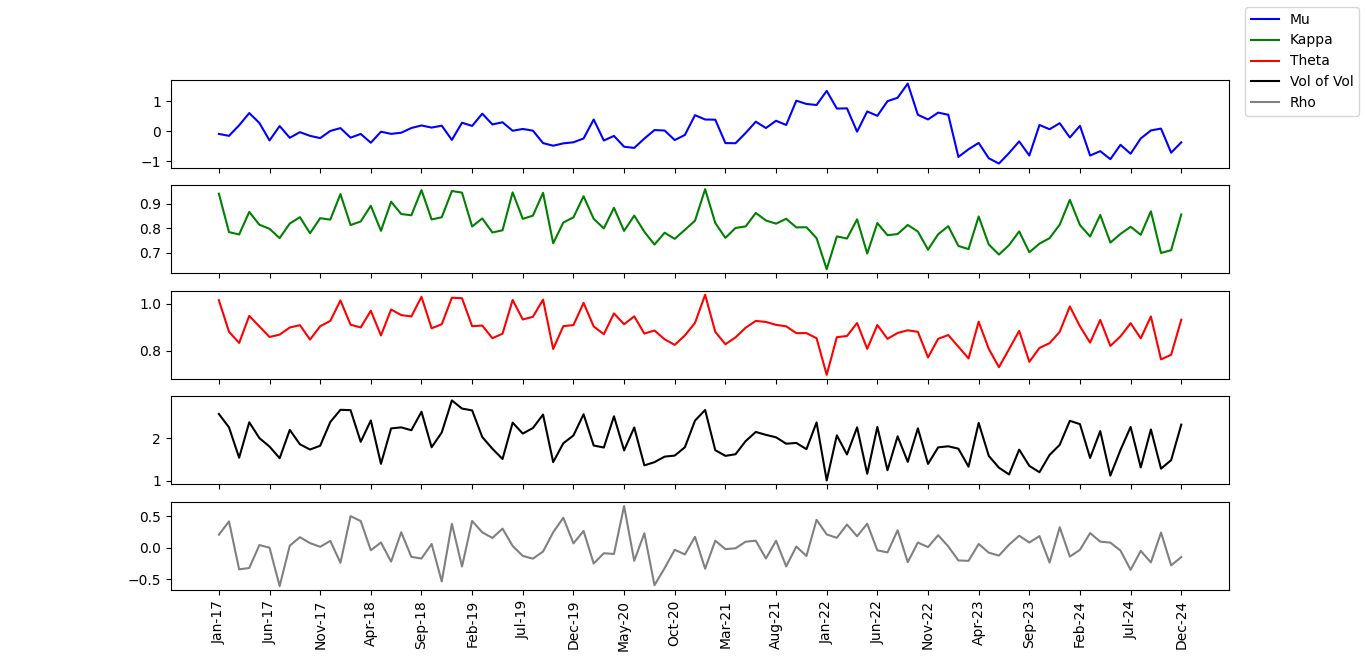
\includegraphics[scale=1,width=1\linewidth,height=0.4\textheight]{heston_params_3m.png}
\caption{Heston parameter estimates from price calibration for 3 month-ahead}
\label{3Mhestonparams}
\end{figure}

\begin{figure}[h!] 
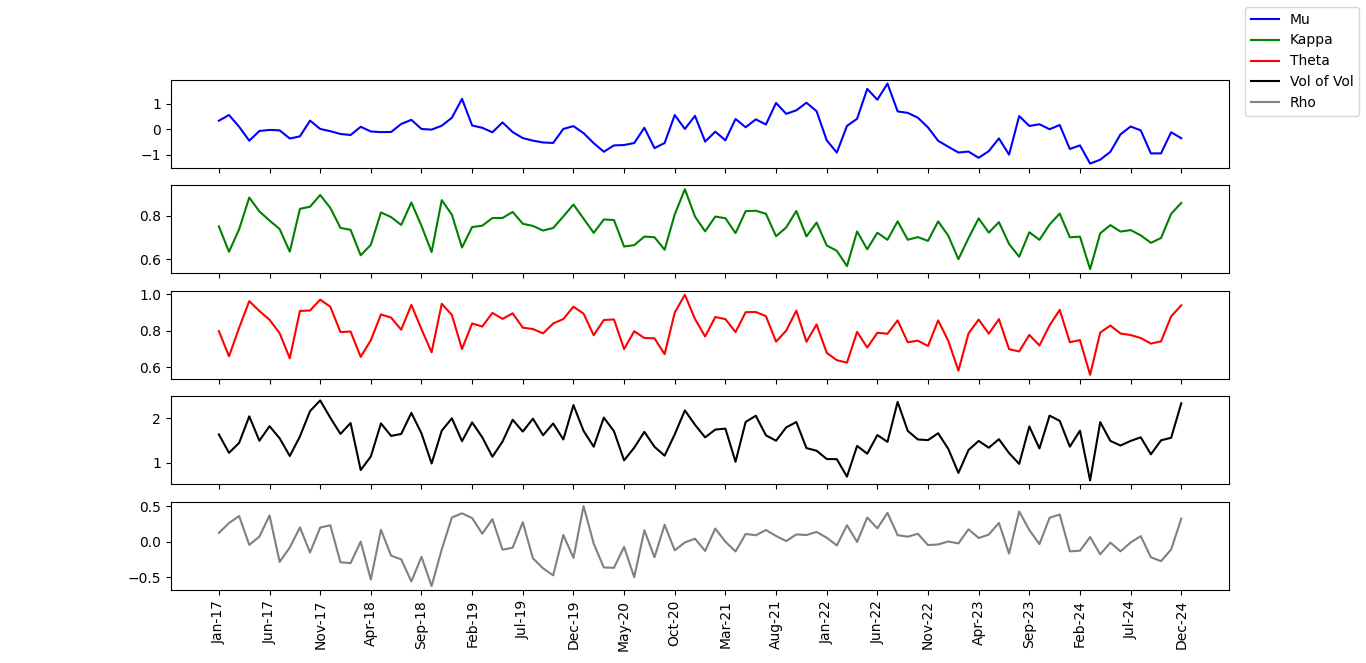
\includegraphics[scale=1,width=1\linewidth,height=0.4\textheight]{heston_params_1m.png}
\caption{Heston parameter estimates from price calibration for 1 month-ahead}
\label{1Mhestonparams}
\end{figure}

EGARCH parameters are shown in \colorAutoref{3Megarchparams} and  \colorAutoref{1Megarchparams}. It is noteworthy from these graphs that both that parameters for 3 month-ahead and 1 month-ahead have the same pattern. Moreover, $\delta$ is 1 implying the symmetric t-distribution for return overtime. 

\begin{figure}[h!] 
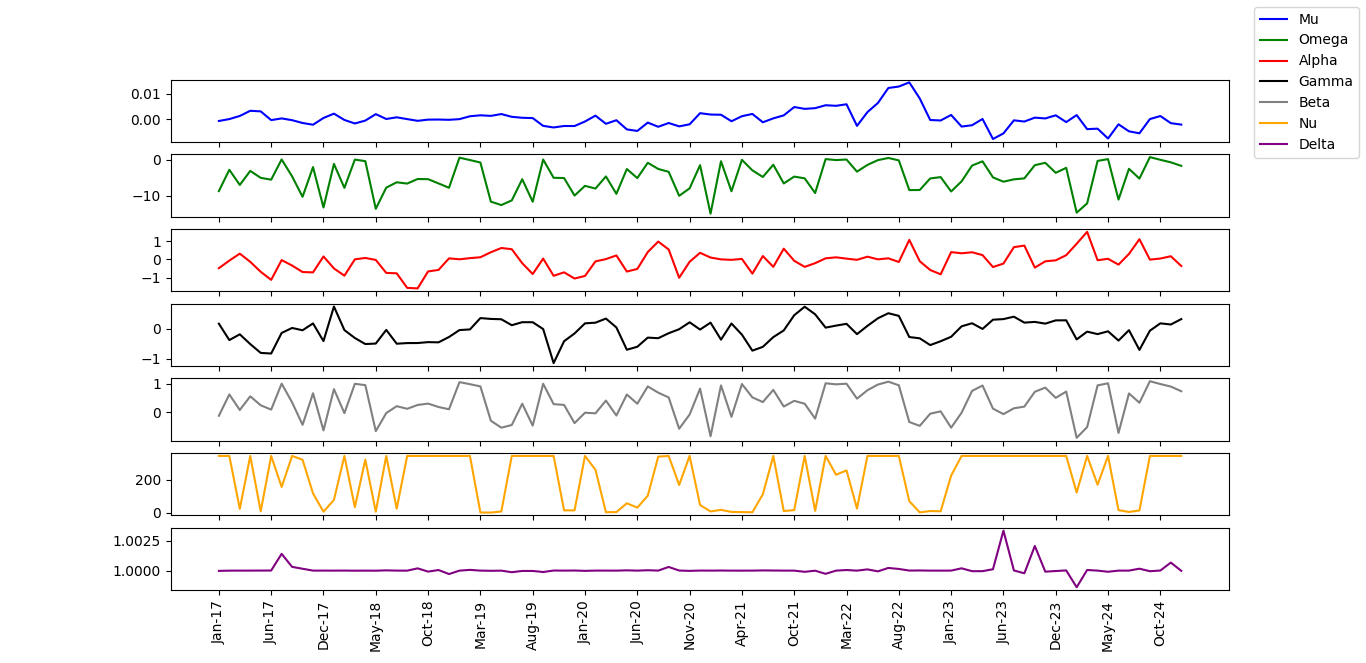
\includegraphics[scale=1,width=1\linewidth,height=0.4\textheight]{egarch_params_3m.png}
\caption{EGARCH parameter estimates from price calibration for 3 month-ahead}
\label{3Megarchparams}
\end{figure}

\begin{figure}[h!] 
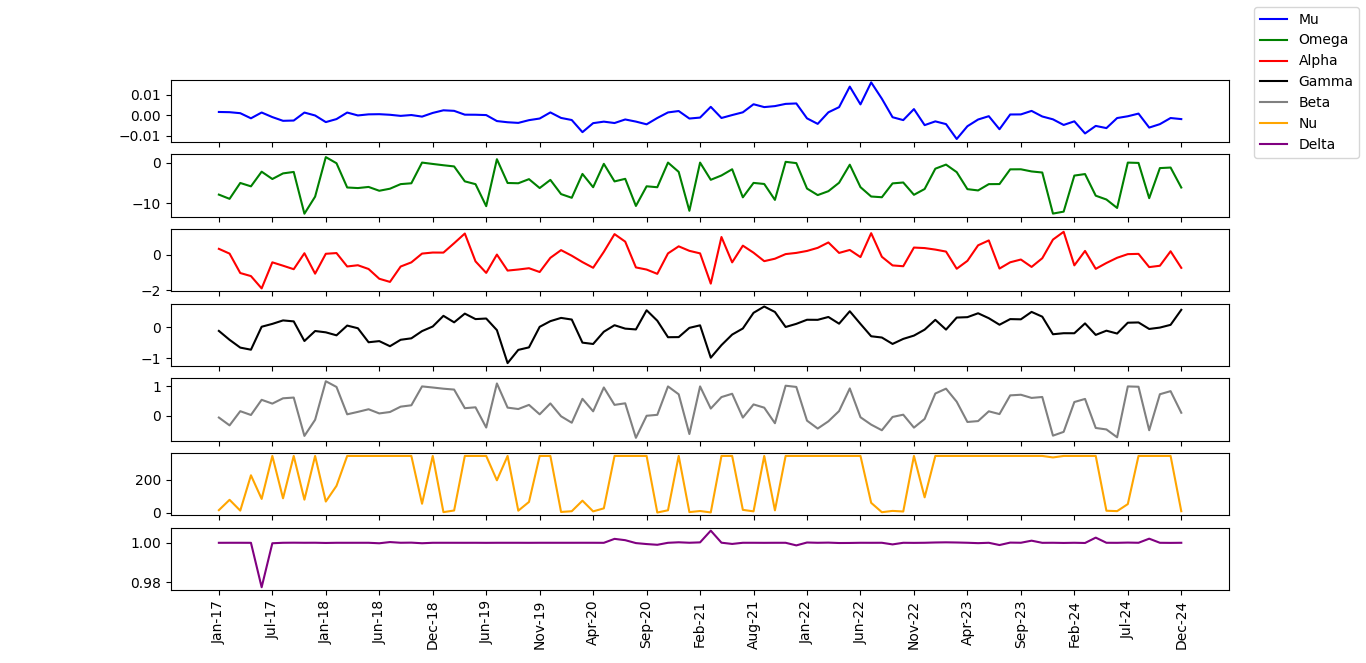
\includegraphics[scale=1,width=1\linewidth,height=0.4\textheight]{egarch_params_1m.png}
\caption{EGARCH parameter estimates from price calibration for 1 month-ahead}
\label{1Megarchparams}
\end{figure}

\subsubsection{In-sample performance}


In-sample CRPS of Heston and EGARCH can be seen from \colorAutoref{3M_in} and \colorAutoref{1M_in} . In general, the fitted distribution of EGARCH is more accurate than the one of Heston, except for the extreme case; e.g, Russian-Ukrainian war 2022. The finding is similar in case of 1 month-ahead forecast where the pattern is found at the beginning of Covid 19. 

\begin{figure}[h!] 
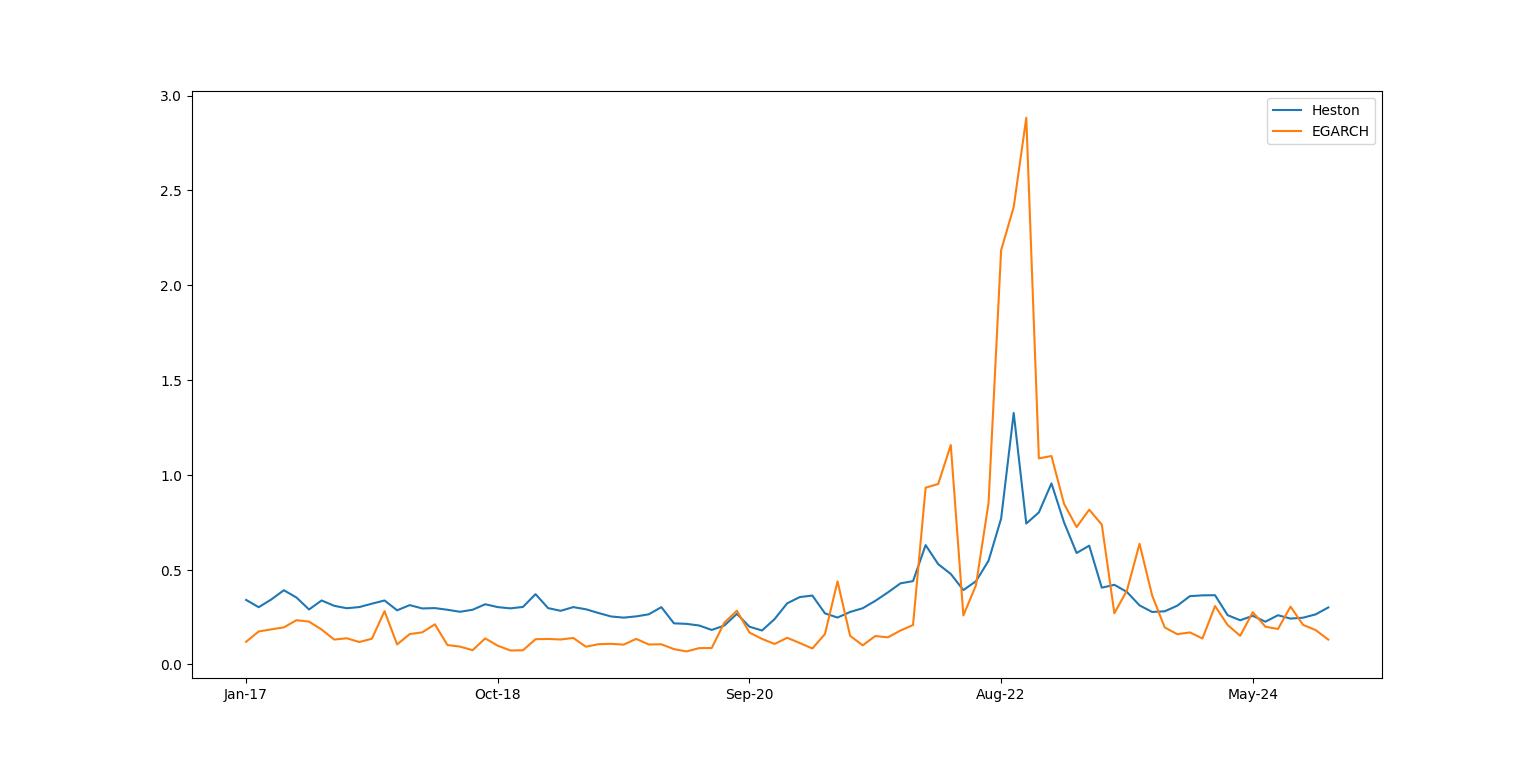
\includegraphics[scale=1,width=1\linewidth,height=0.4\textheight]{insample_crps_3m.png}
\caption{In-sample CPRS of 3 month-ahead models}
\label{3M_in}
\end{figure}

\begin{figure}[h!] 
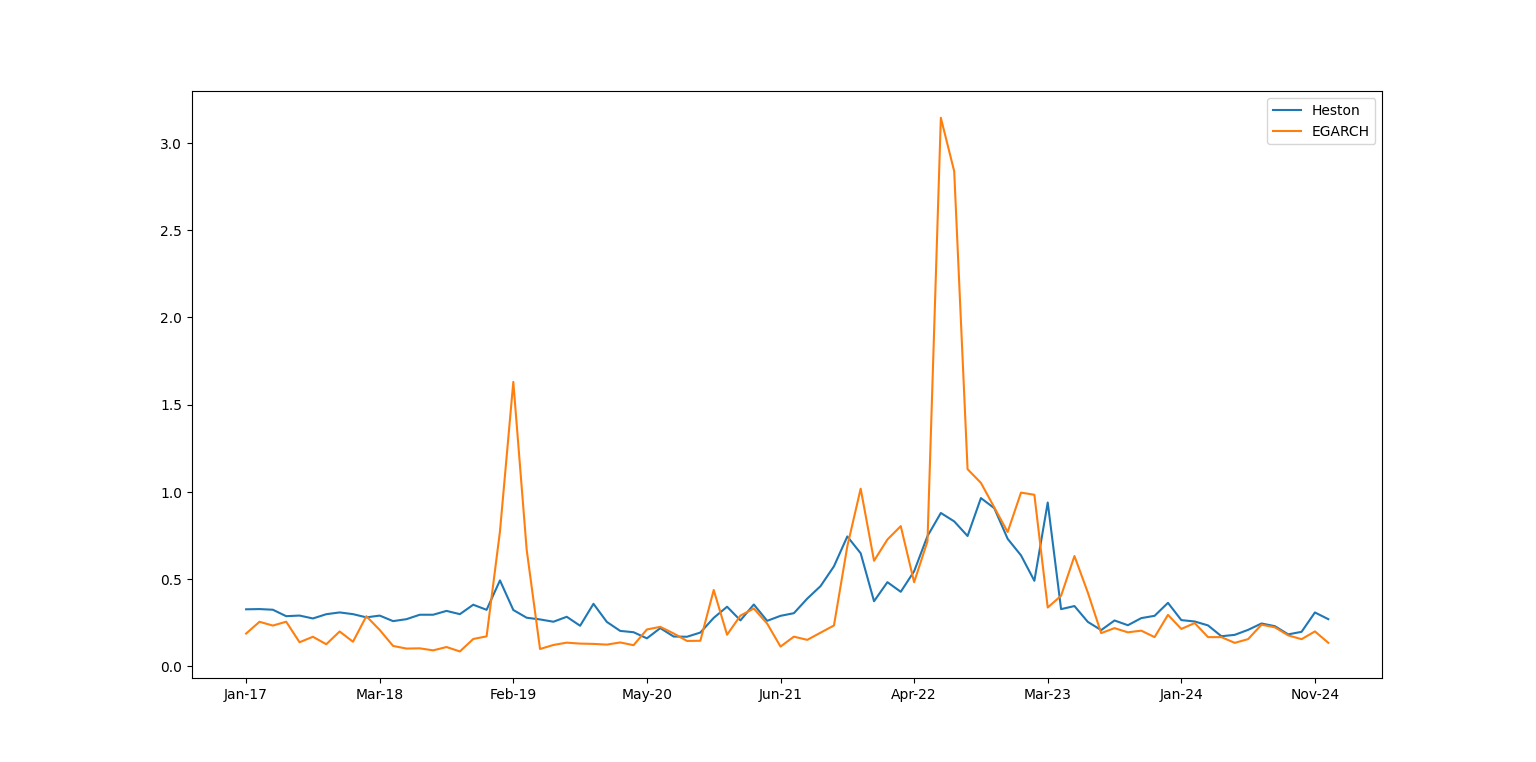
\includegraphics[scale=1,width=1\linewidth,height=0.4\textheight]{insample_crps_1m.png}
\caption{In-sample CPRS of 1 month-ahead models}
\label{3M_in}
\end{figure}

Wilcoxon tests are applied to test the following hypothesis:

H0: The performances of in-sample fitted distribution by Heston and EGARCH model are indifferent.

H1:  In-sample CRPS of EGARCH is smaller than in-sample CRPS of Heston.

\begin{table}[h!]
\centering
\begin{tabular}{@{}lll@{}}
\toprule
N month-ahead     & p-value & Conclusion                     \\ \midrule
3 month-ahead     & 0.0002  & In-sample fitted distribution of EGARCH is more accurate \\
1 month-ahead     & 0.025    & In-sample fitted distribution of EGARCH is more accurate \\ \bottomrule
\end{tabular}
\end{table}

In both forecast scenarios, EGARCH performance is better in terms of in-sample CRPS, which probably suggests the overfitting of EGARCH. The out-sample performance of two models are evaluated in next section in order to examine the forecast accuracy.

\subsection{Predictive performance}

\subsubsection{3 month-ahead forecast}

 In total, data for 96 contracts was used in this study. However, EGARCH model fails at parameterization step for some contracts. In this section, the comparative analysis focuses exclusively on those that both estimated parameters and CPRS are available for both Heston and EGARCH model.
 
 \colorAutoref{3M} shows the forecasting performance of 3 month-ahead models. It can be seen from the \colorAutoref{3M}that in 2022, CRPS of both models are considerably higher than CRPS during the rest of the time. It is clear in \colorAutoref{3Mwithout22} that there is no obvious difference between the CRPS of Heston and EGARCH except for the period of the beginning of Russian-Ukrainian conflict. Moreover, Heston clearly outperform EGARCH during the 2022. In order to have statistical evidence for comparative analysis, non-parametric Wilcoxon tests are run for the whole period without 2022 and for the whole period from 2017 to 2024. 
 

\begin{figure}[h!] 
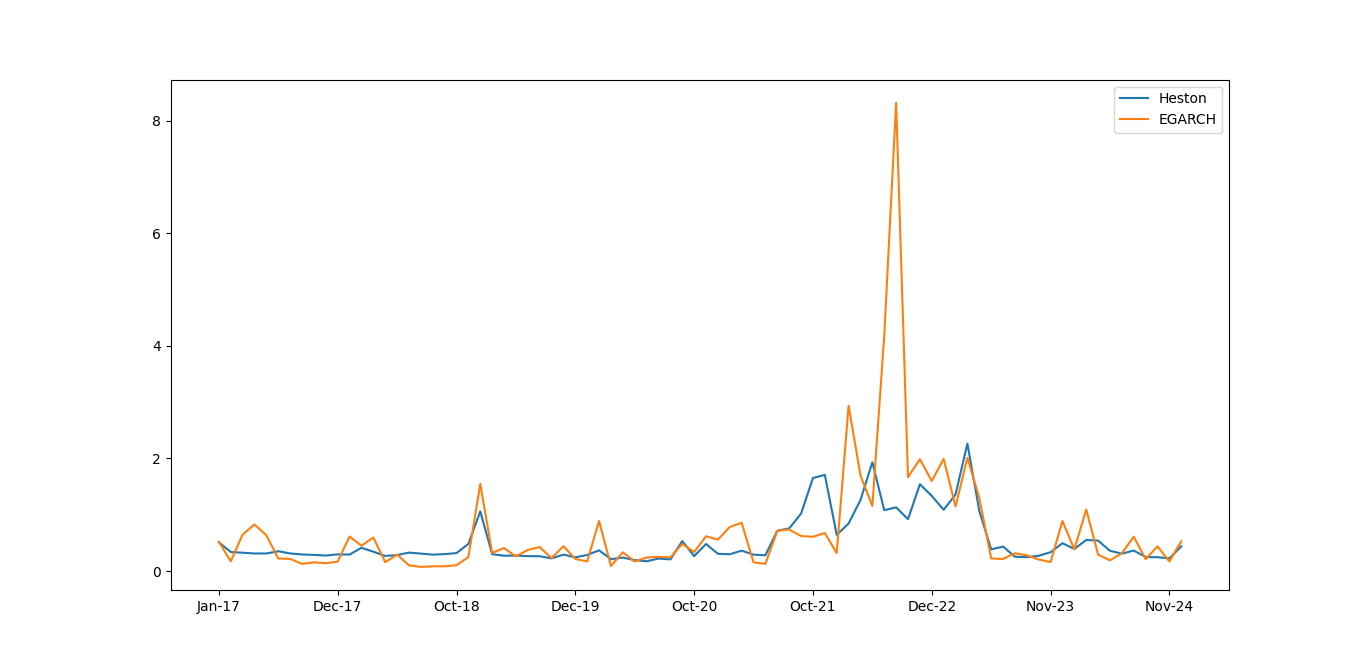
\includegraphics[scale=1,width=1\linewidth,height=0.4\textheight]{threemonthahead.png}
\caption{CPRS of 3 month-ahead models}
\label{3M}
\end{figure}

\begin{figure}[h!] 
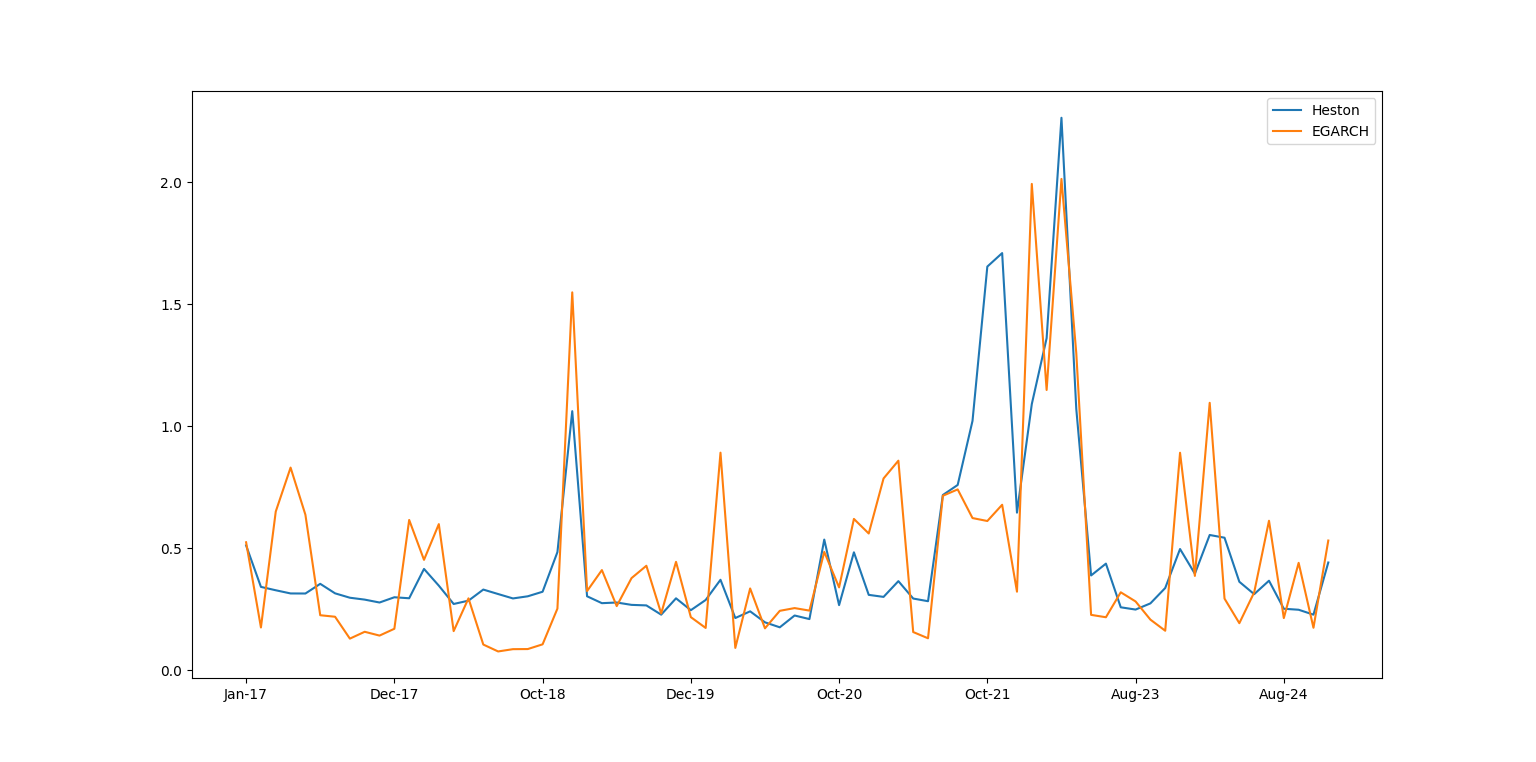
\includegraphics[scale=1,width=1\linewidth,height=0.4\textheight]{m3_without22.png}
\caption{CPRS of 3 month-ahead models excluding 2022}
\label{3Mwithout22}
\end{figure}

Wilcoxon tests are employed to test the following hypothesis:

H0: The performances of Heston and EGARCH model are indifferent.

H1: The performances of 2 models are different.

Table 1 show the result of Wilcoxon tests. In both cases, the null hypothesis is not rejected which means that there is no significant different between the forecasting performance of Heston and EGARCH model for 3 month-ahead forecast.


\begin{table}[h!]
\centering
\begin{tabular}{@{}lll@{}}
\toprule
Investigation period     & p-value & Conclusion                     \\ \midrule
2017-2024                & 0.36    & Fail to reject null hypothesis \\
2017-2024 (without 2022) & 0.88    & Fail to reject null hypothesis \\ \bottomrule
\end{tabular}
\end{table}

CRPS of EGARCH when extreme events happen are noticeably higher than CRPS of Heston model for both in-sample and out-sample for 3 month-ahead forecast. Therefore, even though Heston is computationally expensive and not statistically significant better than EGARCH, one should consider employing HESTON model when there is a concern that an essential event happens unexpectedly. 


\subsubsection{1 month-ahead forecast}

The comparison of CRPS from EGARCH and Heston for 1 month-ahead forecast can be seen from \colorAutoref{1M}. The finding for 1 month-ahead prediction is similar to the one for 3 month-ahead analyzed above, that EGARCH's CRPS is noticeably higher than CRPS of Heston during Covid time in 2019 and Russian-Ukrainian war in 2022. On the other hand, the performance of both models is not dramatically different in terms of CRPS for the rest of the time.

\begin{figure}[h!] 
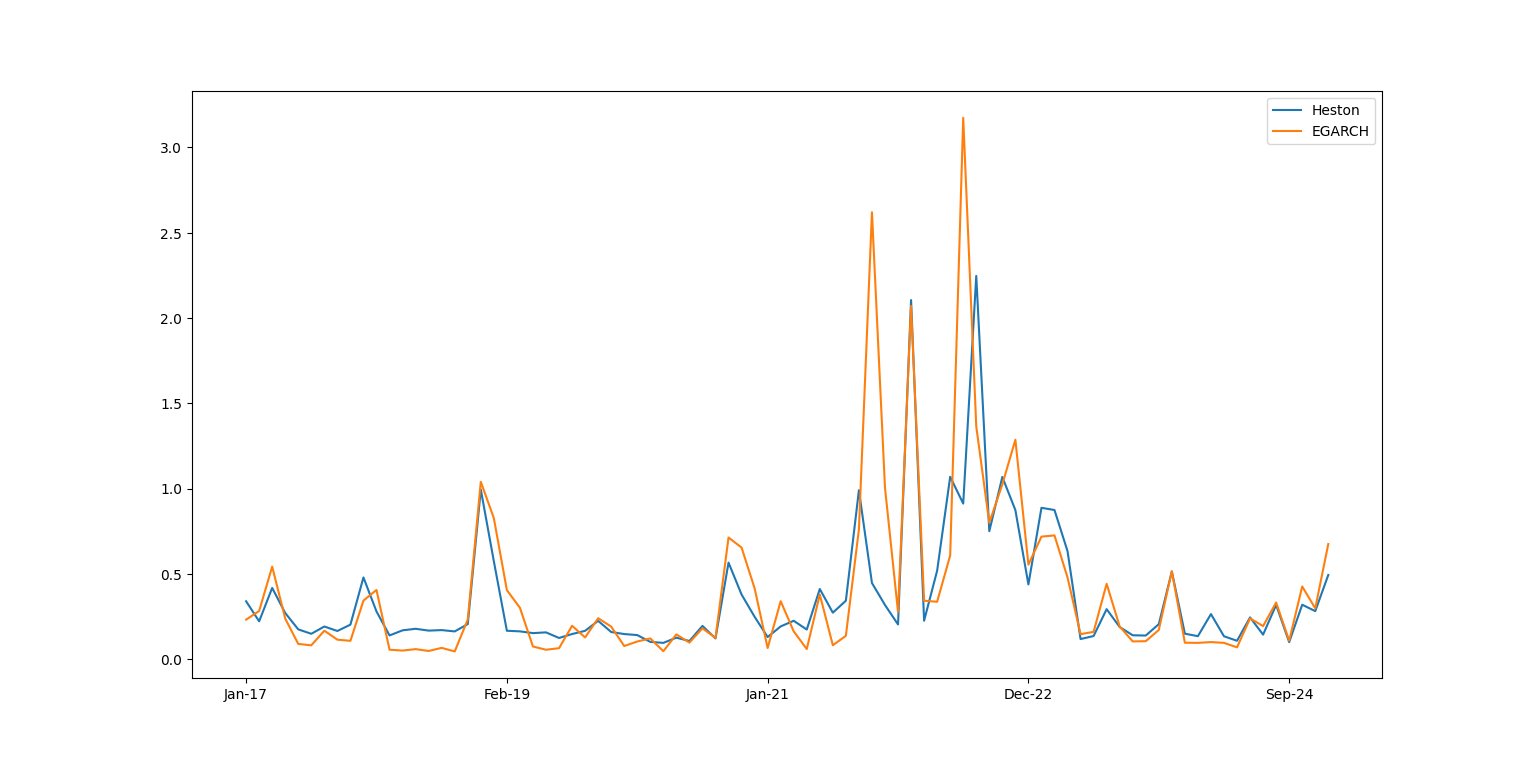
\includegraphics[scale=1,width=1\linewidth,height=0.4\textheight]{onemonthahead.png}
\caption{CPRS of 1 month-ahead models}
\label{1M}
\end{figure}

Two-sided Wilcoxon tests are conducted to investigate the comparison of CRPS from two models, which shows the results as follows:

\begin{table}[h!]
\centering
\begin{tabular}{@{}lll@{}}
\toprule
Investigation period     & p-value & Conclusion                     \\ \midrule
2017-2024                & 0.311    & Fail to reject null hypothesis \\
2017-2024 (without 2022) & 0.186    & Fail to reject null hypothesis \\ \bottomrule
\end{tabular}
\end{table}





\newpage
\section{Conclusion}



\newpage
\begin{thebibliography}{11}
\bibitem{}
Bollerslev, T. (1986). Generalized autoregressive conditional heteroskedasticity.  \emph{Journal of Econometrics}, 31. 307-327.

\bibitem{}
Cape et al. (2014). Estimating Heston's and Bates’ models parameters using Markov chain Monte Carlo simulation.  \emph{Journal of Statistical Computation and Simulation}, 85. 2295-2314.

\bibitem{}
International Energy Agency. (2024). Natural gas demand growth picks up in 2024 amid uncertainties over supply. International Energy Agency. https://www.iea.org/news/natural-gas-demand-growth-picks-up-in-2024-amid-uncertainties-over-supply

\bibitem{}
Energy Information Administration. (2024). Carbon Dioxide Emissions Coefficients. U.S. Department of Energy. https://www.eia.gov/environment/emissions/CO2-vol-mass.php


\bibitem{}

De Gooijer JG, Hyndman RJ (2006). 25 years of time series forecasting. \emph{Int J Forecast}, 22(3). 443-327.


\bibitem{}
Ferrari, D., Ravazzolo, F., \& Vespignani, J. (2021). Forecasting energy commodity prices: A large global dataset sparse approach. \emph{Energy Economics}, 98, 105268.


\bibitem{}
Wang, Y., Liu, L., \& Wu, C. (2020). Forecasting commodity prices out-of-sample: Can technical indicators help?\emph{International Journal of Forecasting}, 36(2), 666–683

\bibitem{}
Sadorsky, P., 1999. Oil price shocks and stock market activity. \emph{Energy Economics}, 21(5), 449–469.

\bibitem{}
Reboredo, J., 2011. How do crude oil prices co-move?: A copula approach. \emph{Energy Economics}, 33(5), 948–955.

\bibitem{}
Engle, R., 1982. Autoregressive conditional heteroscedasticity with estimates of the variance of United Kingdom inflation. \emph{Econometrica: Journal of the econometric society} , 987–1007.

\bibitem{}
Nelson, D., 1991. Conditional heteroskedasticity in asset returns: A new approach. \emph{Econometrica: Journal of the econometric society}, 347–370.

\bibitem{}
Dragulescu, A. A., \& Yakovenko, V. M. (2002). Probability distribution of returns in the Heston model with stochastic volatility. \emph{Quantitative finance}, 2(6), 443.

\bibitem{}
Mikhailov, S., \& Nögel, U. (2004). Heston’s stochastic volatility model: Implementation, calibration and some extensions. \emph{John Wiley and Sons}.

\bibitem{}
Oyuna, D., \& Yaobin, L. (2021). Forecasting the Crude Oil Prices Volatility With Stochastic Volatility Models. \emph{Sage Open}, 11(3)

\bibitem{}
Berrisch, J., \& Ziel, F. (2022). Distributional modeling and forecasting of natural gas prices. \emph{Journal of Forecasting}, 41(6), 1065–1086. 


\bibitem{}
Gruszka, Jarosław, \& Janusz Szwabinski. 2023. Parameter Estimation of the Heston Volatility Model with Jumps in the Asset Prices. \emph{Econometrics}, 11: 15.

\bibitem{}
Cape, J., Dearden, W., Gamber, W., Liebner, J., Lu, Q., \& Nguyen, M. L. (2014). Estimating Heston’s and Bates’ models parameters using Markov chain Monte Carlo simulation. \emph{Journal of Statistical Computation and Simulation}, 85(11), 2295–2314. 





\end{thebibliography}
\newpage
\section*{Appendix}



 
%%%%%%%%%%%%%%%%%%%%%%%%%%%%%%%%%%%%%%%%%%%%%%%%%%%%%%%%%%%%%%%%%%%%%%%%%%%%%%%%%%%%%%%%%%%%
%%%%%%


%\bibliographystyle{apalike}
%\bibliography{Biblio.bib}
%\section*{References}
%\addcontentsline{toc}{section}{References}


%%%%%%%%%%%%%%%%%%%%%%%%%%%%%%%%%%%%%%%%%%%%%%%%%%%%%%%%%%%%%%%%%%%%%%%%%%%%%%%%%%%%%%%%%%%%%%%%%%

\setcounter{equation}{0}
\renewcommand\theequation{\Alph{section}.\arabic{equation}}	
\setcounter{table}{0}
\renewcommand\thetable{\Alph{section}.\arabic{table}}
\setcounter{figure}{0}
\renewcommand\thefigure{\Alph{section}.\arabic{figure}}




\end{document}